%% Springer Nature sn-jnl template (December 2024)
%% Style: JASM published two-column layout, Math and Physical Sciences numbered references
\documentclass[pdflatex,sn-mathphys-num,twocolumn]{sn-jnl}

\usepackage{amsmath,amssymb,amsfonts}
\usepackage{algorithm}
\usepackage{algorithmic}
\usepackage{graphicx}
\usepackage{textcomp}
\usepackage{xcolor}
\usepackage{booktabs}
\usepackage{multirow}
\usepackage{enumitem}
\usepackage{hyperref}
\usepackage{tikz}
\usepackage{pgfplots}
\pgfplotsset{compat=1.18}
\usepackage{bm}
\usepackage{adjustbox}
\usepackage{float}
\setlist{nosep,leftmargin=*}

%% Override sn-jnl single-column geometry for proper two-column layout
\geometry{
  a4paper,
  top=18mm, bottom=20mm,
  inner=18mm, outer=14mm,
  columnsep=5mm,
  textwidth=178mm,
  textheight=255mm,
  headheight=12pt, headsep=5mm,
  footskip=10mm
}
\setlength{\columnsep}{5mm}

%% Theorem styles provided by sn-jnl.cls
\theoremstyle{thmstyleone}
\newtheorem{proposition}{Proposition}
\theoremstyle{thmstyletwo}
\newtheorem{heuristic}{Heuristic Analysis}
\newtheorem{remark}{Remark}

% MOS figure colour palette (colorblind-safe)
\definecolor{cHuman}{RGB}{70,90,110}
\definecolor{cPF}   {RGB}{31,119,180}
\definecolor{cMGen} {RGB}{44,160,44}
\definecolor{cTM}   {RGB}{196,78,82}
\usetikzlibrary{shapes.geometric, arrows, positioning, fit, calc}

% Unified significance legend
\newcommand{\siglegend}{\vspace{2pt}{\scriptsize
  $^{*}p{<}0.05$;\;$^{**}p{<}0.01$;\;$^{***}p{<}0.001$;\;{\itshape n.s.} not sig.\;
  All pairwise vs.\ \textbf{PulseFormer}, Mann--Whitney~$U$ (two-sided, Bonferroni corrected).}}

\raggedbottom
\setlength{\textfloatsep}{8pt plus 2pt minus 2pt}
\setlength{\floatsep}{8pt plus 2pt minus 2pt}
\setlength{\intextsep}{7pt plus 2pt minus 2pt}
\setlength{\dbltextfloatsep}{8pt plus 2pt minus 2pt}
\setlength{\dblfloatsep}{8pt plus 2pt minus 2pt}
\setlength{\abovecaptionskip}{4pt}
\setlength{\belowcaptionskip}{2pt}
\setlength{\tabcolsep}{3pt}
\renewcommand{\arraystretch}{0.92}

\begin{document}

\title{PulseFormer: A Hybrid Controllable Music-Processing Pipeline for DAW-Oriented Multi-Track Electronic Music Generation}

\author*[1]{\fnm{Zhenyu} \sur{Xiong}}\email{yaralastudio@shu.edu.cn}
\author[1]{\fnm{Yonghua} \sur{Zhu}}\email{zyh@shu.edu.cn}

\affil*[1]{\orgdiv{Shanghai Film Academy}, \orgname{Shanghai University}, \orgaddress{\city{Shanghai}, \country{China}}}

\abstract{This paper presents PulseFormer, a hybrid music-processing pipeline for structure-guided, controllable multi-track Electronic Music generation tailored to Digital Audio Workstation (DAW) production workflows. The system addresses two practical limitations of prior symbolic MIDI models: high representational burden when coordinating simultaneously active instruments in dense arrangements and limited control over section-level density progression.

PulseFormer combines three engineering choices. First, a Time-Major compound-token representation places concurrent cross-track events close together in the autoregressive sequence, reducing the token-distance burden for modelling kick, bass, chord, and melodic co-activation. Second, a structural density identifier, $\mathbf{E}_{\mathrm{level}}$, encodes the track-stacking intensity of each section (Intro, Buildup, Drop, Breakdown, Outro). This identifier conditions generation through both a prefix token and Feature-wise Linear Modulation (FiLM), which applies learned scale-shift transformations at every Transformer layer. Third, Temporal Anchor Stitching assembles section-wise generations into long-form arrangements beyond the model context window while retaining editable stems.

Experiments show that PulseFormer achieves the highest qualified-note rate among trained models ($42.5\%$). FiLM improves local 8-bar structural density response from $r=0.155$ to $r=0.997$; at pipeline scale, the joint model-plus-Scheduler Pearson correlation over 128-bar arrangements is $r=0.982$, which is interpreted as hybrid target adherence rather than fully learned long-form planning. Beat-level alignment is comparable across trained systems, harmonic diversity is similar, and groove consistency remains lower than the Track-Major baseline. A rendered-audio MOS protocol provides perceptual support but is not treated as distribution-level proof of overall musical-quality superiority. These results position PulseFormer as a production-oriented music-processing framework for controllable section-level density, rendered listening evaluation, and editable DAW stem generation.}

\keywords{Audio and Music Processing, Symbolic Music Generation, Transformer, Multi-track Composition, Structural Density Control, Electronic Music}

\maketitle

\section{Introduction}
\begin{figure*}[!t]
\centering
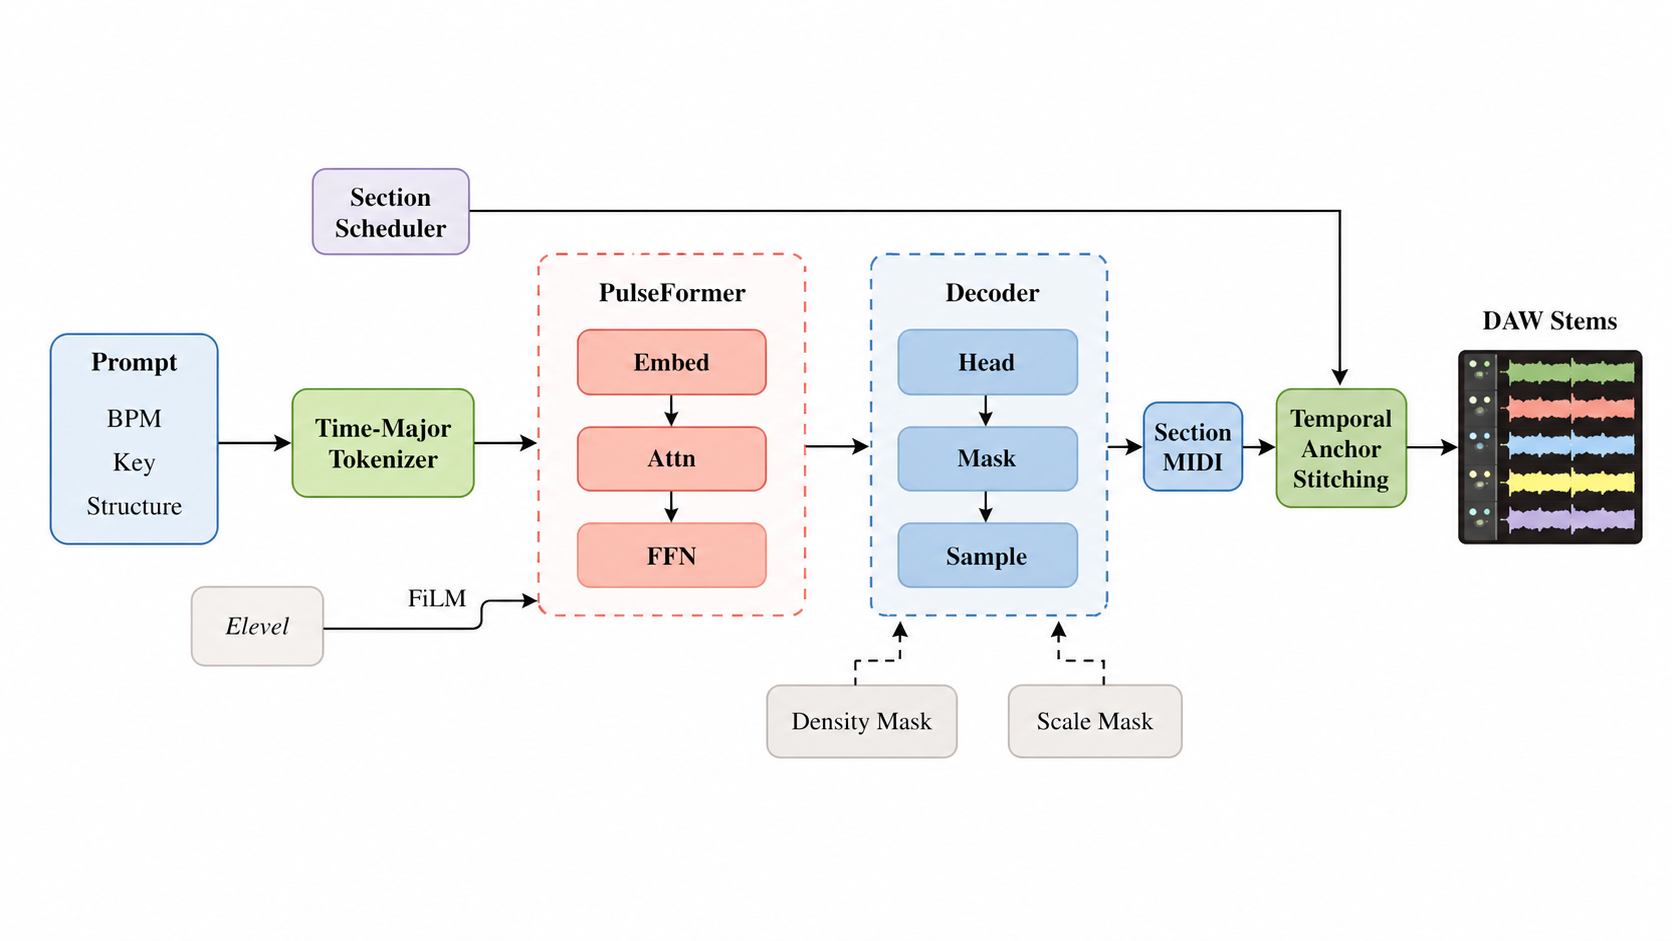
\includegraphics[width=\linewidth]{figures/architecture_new.png}
{\sloppy\hbadness=10000\caption{PulseFormer System Architecture. The system integrates structural conditioning, Time-Major tokenization, and temporal anchor stitching for multi-track DAW stem generation.\label{fig:pipeline}}}
\end{figure*}
Deep generative architectures have been applied across a range of creative domains, including visual synthesis and audio waveform generation~\cite{dhariwal2020jukebox, donahue2023singsong}. Audio-domain models trained on large corpora have achieved strong timbral realism; however, symbolic-domain music generation (i.e., MIDI sequencing) remains relevant for music-processing workflows in which structural transparency, per-track editability, rendered-audio validation, and DAW interoperability are practical requirements~\cite{huang2019music, payne2019musenet, dong2020muspy}.

While existing symbolic music generation models have achieved promising results, their performance in rhythmically dense Electronic Music settings remains limited. In particular, when multiple instruments are activated simultaneously, large token distances between concurrent events increase the representational burden for cross-track coordination. Additionally, most autoregressive models provide limited mechanisms for explicitly controlling the structural density progression of multi-track arrangements across musical sections.

Although prior work has explored various token representations and conditioning strategies, the impact of representation topology on local cross-track coordination in dense multi-track settings remains underexplored. Furthermore, controllable generation of structural density trajectories aligned with DAW section structures (Intro, Buildup, Drop, Breakdown, Outro) in symbolic music remains an open challenge, particularly in production-oriented workflows that must ultimately be rendered, normalized, auditioned, and edited as audio stems.

This paper introduces \textbf{PulseFormer}, a domain-targeted music-processing pipeline designed specifically for Electronic Music production. Rather than proposing a general-purpose music generation architecture, PulseFormer makes deliberate engineering choices---Time-Major token ordering, structural-density conditioning, section-by-section generation, and DAW-oriented rendering/export---that are well-suited to the rhythmically strict, layered structure of Techno and House music, but entail explicit trade-offs discussed in Section~\ref{sec:conclusion}. 

The principal contributions of this paper are summarized as follows:
\begin{enumerate}
    \item \textbf{Structural Density Conditioning via FiLM}: We introduce a structural density control identifier, $\mathbf{E}_{\mathrm{level}} \in \{1,\ldots,8\}$, derived from an empirically calibrated 6-feature score $D_t$ that quantifies per-bar polyphonic track-stacking intensity. This identifier is directly aligned with DAW production conventions: low values correspond to sparse Intro textures, mid values to Buildup sections, and high values to dense Drop arrangements. $\mathbf{E}_{\mathrm{level}}$ conditions the model via a \emph{dual-pathway} mechanism: (i) as a sequence-level prefix token that anchors early attention patterns to the section identity, and (ii) through Feature-wise Linear Modulation (FiLM;~\cite{perez2018film}), which applies per-layer learned affine transformations $(\boldsymbol{\gamma}_\ell, \boldsymbol{\beta}_\ell)$ to every Transformer layer's output, ensuring persistent depth-wide modulation. Together with an external section scheduler, this mechanism improves \emph{local} structural density trajectory adherence from $r=0.155$ to $r=0.997$ on 8-bar sequences (Pearson $r$ against the target density ramp; \S~\ref{sec:ablation}). At pipeline scale, the joint model-plus-Scheduler Pearson $r$ over 128-bar arrangements is $r=0.982$. These two figures measure qualitatively distinct properties: the first isolates FiLM's \emph{local conditioning fidelity} on held-out validation sequences; the second reflects the combined \emph{macro-structural enforcement} of FiLM and the deterministic Ramp Scheduler over full-length arrangements and should be interpreted as hybrid model-plus-rule behaviour, not as fully end-to-end learned long-form planning.
    \item \textbf{Time-Major Coordination Topology}: We propose a compound event representation ordered chronologically across the full arrangement, with five independently predicted dimensions (type, pitch, position, duration, velocity) unified into a single compound token via Time-Major serialization. Co-locating concurrent instruments within a narrow token window ($\leq\!12$ tokens) reduces the mean co-event token distance from $\approx\!3{,}268$ tokens (Track-Major) to $5.2$ tokens. We interpret this as reducing the representational burden for local cross-track coordination; output-level synchronization evidence is reported cautiously because several timing metrics are partly determined by quantized representation and DAW post-processing.
    \item \textbf{Temporal Anchor Stitching}: Because Time-Major interleaving increases token density, the effective context window covers only $\sim$8 bars per generation batch. This limitation is addressed by a batch-level stitching procedure in which each new section is initialized with the final $k$ bars of the preceding section as a shared prefix anchor, preserving rhythmic grid alignment across section boundaries. This approach extends arrangement length to $128+$ bars but does not provide full end-to-end long-context memory; cross-section melodic coherence degrades over extended windows, a limitation discussed in Section~\ref{sec:conclusion}.
\end{enumerate}

Fig.~\ref{fig:pipeline} provides a high-level system overview of the complete PulseFormer generation pipeline.




\section{Related Work}
\label{sec:related_work}

Symbolic multi-track music generation has progressed from GAN-based piano-roll models~\cite{dong2018musegan} to Transformer architectures~\cite{huang2019music, huang2020remi} with compound-token representations~\cite{hsiao2021compound, zeng2021musicbert} that compress note attributes into multi-dimensional embeddings. Track-Major serialization (MMM~\cite{ens2020mmm}, LakhNES~\cite{donahue2019lakhnes}) separates instruments into sequential blocks; this increases token distance between concurrent cross-track events, which may hinder synchronization in dense polyphonic settings.
For controllability, audio-domain systems (MusicGen~\cite{copet2023simple}, MusicLM~\cite{agostinelli2023musiclm}) accept text prompts but produce unquantized waveforms unsuitable for per-stem DAW editing. In the symbolic domain, FIGARO~\cite{von2022figaro} and MuseMorphose~\cite{wu2023musemorphose} condition on high-level descriptors; BandControlNet~\cite{luo2024bandcontrolnet} uses fine-grained spatiotemporal features for multi-instrument control. PulseFormer differs by using an explicit track-stacking ordinal identifier conditioned via FiLM and a deterministic section scheduler, targeting DAW-production workflows.

\section{Methodology}
\label{sec:methodology}


\subsection{Architecting the Time-Major Compound Token Space}
Unlike sequential language models operating on rigid single-dimensional vocabulary indices, musical events encompass distinct yet intersecting modalities (instrument classification, pitch, duration, and acoustic velocity). Following Compound Word (CP)~\cite{hsiao2021compound} semantics, PulseFormer represents each discrete musical event $x_i$ as a unified compound token with five independently predicted dimensions---instrument type, pitch, bar-position, duration, and velocity---embedded and summed as:
\begin{equation} \label{eq:embedding}
E(x_i) = \sum_{F \in \mathcal{F}} W_F(\text{id}_F(x_i))
\end{equation}
where $\mathcal{F} = \{Type, Pitch, Position, Duration, Velocity\}$. Position encodes the 16th-note grid step within a bar ($v^{\mathrm{pos}}\in\{0,\dots,15\}$) and is predicted as an independent compound dimension alongside the four note-attribute fields.
The concrete vocabulary assigned to each field is listed in Table~\ref{tab:vocab}.

\begin{tableorg}[ht]
\centering\small
\caption{Vocabulary sizes for the Time-Major 5-dimensional compound token
  representation. Each musical event is encoded as a tuple
  $(v^{\mathrm{type}}, v^{\mathrm{pitch}}, v^{\mathrm{pos}}, v^{\mathrm{dur}}, v^{\mathrm{vel}})$
  with independent prediction heads per dimension.
  All values are derived from the \textsc{pulse\_dataset\_v6} training corpus.}
\label{tab:vocab}
\adjustbox{max width=\columnwidth}{
\begin{tabular}{@{}llrp{5cm}@{}}
\toprule
\textbf{Field} & \textbf{Symbol} & \textbf{$|V_F|$} & \textbf{Range / notes} \\ \midrule
Instrument type & $v^{\mathrm{type}}$ & 10
  & \texttt{BASS, CHORD, MELODY, DRUMS} (instrument classes)
    $+$ \texttt{GLOBAL, BAR} (structural tags)
    $+$ \texttt{PAD, BOS, EOS, NONE} \\ \midrule
Pitch / attribute & $v^{\mathrm{pitch}}$ & 234
  & Pitch names (\texttt{C3}\ldots\texttt{B6}), drum labels
    (\texttt{KICK}, \texttt{SNARE}, \texttt{HIHAT\_*}), and global attribute
    values (\texttt{STRUCT\_DROP}, \texttt{KEY\_C\_MINOR},
    \texttt{BPM\_128}, \texttt{ENERGY\_LEVEL\_*}, \ldots) \\ \midrule
Step position    & $v^{\mathrm{pos}}$ & 20
  & 16th-note grid steps $0$--$15$ within a bar,
    plus 4 special tokens \\ \midrule
Duration         & $v^{\mathrm{dur}}$ & 10
  & $\{1, 2, 4, 8, 16\}$ (16th-note units, clipped per track type)
    $+$ 5 special tokens \\ \midrule
Velocity         & $v^{\mathrm{vel}}$ & 8
  & Bins $v_0$--$v_3$ (equal-width MIDI bins)
    $+$ 4 special tokens \\
\midrule
Control tags & \multicolumn{2}{r}{in $v^{\mathrm{pitch}}$}
  & \texttt{[STRUCT\_\{INTRO, BUILDUP, DROP,} \newline
    \texttt{BREAKDOWN, OUTRO, PATTERN\}]}; \newline
    \texttt{[ENERGY\_LEVEL\_1..8]}; \texttt{[KEY\_*]}; \newline
    \texttt{[BPM\_*]}; \texttt{[BAR\_*]}; \texttt{[HAS\_*]} \\
\bottomrule
\end{tabular}
}
\end{tableorg}

The model uses 6 Transformer layers, 8 attention heads, $d=512$, SwiGLU FFN ($d_{\mathrm{ff}}=1{,}376$), and per-layer FiLM modules, totalling \textbf{24.0\,M} parameters. Baselines use the same architecture without FiLM (${\approx}19.8\,\mathrm{M}$). Rather than Track-Major serialization, PulseFormer enforces \textbf{Time-Major Interleaving}: concurrent events across instruments occupy adjacent token positions (cross-track distance $\Delta \leq M$, $M\leq8$ tracks), compared to a mean of 3{,}249 tokens under Track-Major (Table~\ref{tab:attention}).

\subsection{Causal Transformer Architecture}
PulseFormer employs a decoder-only causal Transformer~\cite{vaswani2017attention} with FlashAttention~\cite{dao2022flashattention}:
$A = \operatorname{Softmax}\!\left({QK^\top}/{\sqrt{d_k}} + M\right)V$, $M_{ij}=-\infty\;\forall j>i$.

\subsection{FiLM Conditioning: Energy-Level Modulation}
\label{sec:film}
Feature-wise Linear Modulation (FiLM)~\cite{perez2018film} provides depth-wide conditioning of the Transformer on the structural density level $\mathbf{E}_{\mathrm{level}}$. After the multi-head attention and feed-forward sublayers of each Transformer layer $\ell$, FiLM applies a learned affine transformation to the entire hidden sequence:
\begin{equation}\label{eq:film}
  \tilde{h}_\ell = \boldsymbol{\gamma}_\ell(\mathbf{E}_{\mathrm{level}}) \odot h_\ell
                 + \boldsymbol{\beta}_\ell(\mathbf{E}_{\mathrm{level}}),
\end{equation}
where $h_\ell \in \mathbb{R}^{T \times d}$ is the layer output and $\boldsymbol{\gamma}_\ell,\boldsymbol{\beta}_\ell \in \mathbb{R}^d$ are scale and shift vectors produced by a two-layer MLP:
\begin{equation}\label{eq:film_mlp}
  [\boldsymbol{\gamma}_\ell;\,\boldsymbol{\beta}_\ell]
    = W_\ell^{(2)}\,\sigma\!\left(W_\ell^{(1)}\,e(\mathbf{E}_{\mathrm{level}})+b_\ell^{(1)}\right)+b_\ell^{(2)},
\end{equation}
with $e:\{1,\dots,8\}\!\to\!\mathbb{R}^d$ a learned energy-level embedding and $\sigma$ the SiLU activation. The FiLM MLPs are shared across the time dimension but applied independently per layer, contributing $|\theta_{\mathrm{FiLM}}|\approx4.2\,\mathrm{M}$ parameters to the 24.0\,M total.

The \textbf{dual-pathway} conditioning combines a prefix token (sequence-level anchor in early attention layers) with FiLM (layer-level re-injection at every depth), preventing density-signal decay across layers.

\subsection{Inference Pipeline}
At inference time, the token-level probability distribution of the Transformer is modified by two deterministic masks applied prior to sampling: an Energy Density mask (which gates high-velocity note tokens when the current bar count exceeds the $\mathbf{E}_{level}$ polyphony budget) and a Diatonic Scale mask (described in Section~\ref{sec:soft_mask}). Algorithm~\ref{alg:pulseformer} presents the complete per-step procedure.

\begin{algorithm*}[!t]
\caption{PulseFormer Steerable Multi-Track Inference}
\label{alg:pulseformer}
\begin{algorithmic}[1]
\REQUIRE Pre-trained model $\Theta$, Temperature $\tau$, Prompt $\mathcal{C}$, Energy level $\mathbf{E}_{\mathrm{level}}$, Max Tokens $T_{\max}$
\STATE Initialize sequence canvas $X \leftarrow \mathcal{C}$
\FOR{$t = 1$ to $T_{\max}$}
    \STATE Compute hidden states layer by layer:
    \FOR{$\ell = 1$ to $L$}
        \STATE $h_\ell \leftarrow \text{TransformerLayer}_\ell(h_{\ell-1})$ \hfill\COMMENT{attention + FFN}
        \STATE $\tilde{h}_\ell \leftarrow \boldsymbol{\gamma}_\ell(\mathbf{E}_{\mathrm{level}}) \odot h_\ell + \boldsymbol{\beta}_\ell(\mathbf{E}_{\mathrm{level}})$ \hfill\COMMENT{FiLM modulation; $\tilde{h}_\ell$ per Eq.~\eqref{eq:film}}
    \ENDFOR
    \STATE Project into raw logits over compound event vocabulary: $z^{(t)} \leftarrow W \cdot h_L[-1]$
    \FORALL {$k \in \mathcal{V}$}
        \IF{$\mathbf{E}_{level}$ restricts polyphony density limit $D_{\max}$}
            \STATE Apply density algorithmic mask $M_{energy} \to z_k^{(t)}$
        \ENDIF
        \IF{Diatonic constraint active \AND Type is Pitch}
            \STATE Apply pitch mask $M_{scale} \leftarrow -\infty$ to $z_k^{(t)}$ if outside Key
        \ENDIF
    \ENDFOR
    \STATE Compute probability vector $P \leftarrow \text{Softmax}(z^{(t)} / \tau)$
    \STATE Sample new compound event token $e_t \sim P$
    \STATE Append $X \leftarrow X \oplus e_t$
\ENDFOR
\RETURN Generated multi-track sequence array $X$
\end{algorithmic}
\end{algorithm*}

\subsection{Structural Density Conditioning \& Section-Level Scheduling}
\label{sec:cond}
A hierarchical prompt $\mathcal{C} = [\mathcal{S}_{struct},\,\mathbf{E}_{level},\,\mathcal{K}_{key},\,\mathcal{T}_{bpm}]$ conditions every autoregressive phase. Genre conditioning is deliberately omitted: the training corpus spans heterogeneous Electronic Music subgenres that cannot be reliably labelled at fine granularity, and genre-specific generation is delegated to a downstream arrangement-control layer. The joint generation distribution is:
\begin{align}
P(X_{1:T}\mid\mathcal{C},\mathbf{E}_{\mathrm{level}})
  &= \prod_{t=1}^{T}
     \!\left[\operatorname{Softmax}\!\left(\tfrac{W_o\,\tilde{h}_t+b_o}{\tau}\right)\right]_{x_t},
\end{align}
where $\tilde{h}_t \triangleq \tilde{h}_L(X_{<t},\mathcal{C},\mathbf{E}_{\mathrm{level}})$ is the FiLM-modulated final hidden state (Eq.~\eqref{eq:film}), and $[\cdot]_{x_t}$ selects the probability of the actual token $x_t$.

$\mathbf{E}_{level}\in\{1,\dots,8\}$ is a structural density control identifier that encodes the per-section polyphonic track-stacking intensity. It does not represent a psychoacoustic energy quantity; rather, it directly corresponds to the Intro-Buildup-Drop layer accumulation logic of DAW production practice: level~1 maps to sparse Intro textures (few active tracks), levels~4--6 to Buildup sections (incrementally stacked layers), and levels~7--8 to full Drop arrangements (all tracks active at high velocity). The model conditions on this identifier through the dual-pathway mechanism described in \S~\ref{sec:film} (prefix token + FiLM), but does not learn long-range density trajectories across sections. Full-length arrangements are assembled externally: each section is generated independently with its assigned $\mathbf{E}_{\mathrm{level}}$, then joined by the Temporal Anchor Stitching procedure (Section~\ref{sec:stitching}). Structural density monotonicity across sections is therefore an \textbf{algorithmic scheduling mechanism}, not an emergent model property.

\begin{figure*}[!t]
\centering
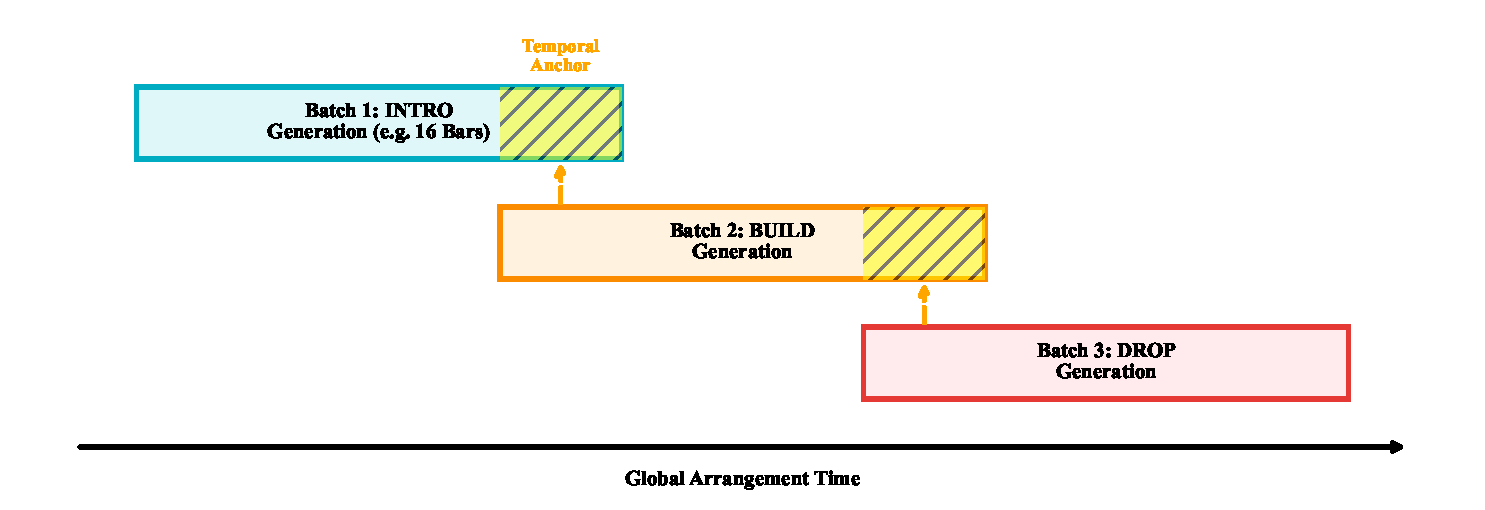
\includegraphics[width=0.88\linewidth, trim=0 20pt 0 20pt, clip]{figures/stitching.pdf}
\caption{Section-level scheduling pipeline. Each structural section is generated independently under its own $\mathbf{E}_{\mathrm{level}}$ prefix; the Temporal Anchor Stitching procedure concatenates sections at the engineering level. Structural density monotonicity is a property of the external scheduler, not the Transformer.}
\label{fig:macro_pipeline}
\end{figure*}

\subsection{Temporal Anchor Stitching}
\label{sec:stitching}
To exceed the 2048-token context window, section transitions retain the final $K$ beats of the preceding segment in the KV-cache and apply a linear time offset:
\begin{equation}
\mathrm{TimePos}_{N+1} = \mathrm{TimePos}_N + \Delta T_{\mathrm{offset}}.
\end{equation}
At section boundaries with a discrete density jump $\Delta E = |E_{\mathrm{dst}}-E_{\mathrm{src}}|$, abrupt tag changes can produce audible density discontinuities. The Active Density Ramp Scheduler addresses this by inserting $W$ single-bar intermediate sections with linearly or smoothly interpolated tags:
\begin{align}
E_k &= \mathrm{clip}\!\bigl(\mathrm{round}(E_{\mathrm{src}}+\Delta E\cdot\phi(k/W)),\;1,\;8\bigr), \nonumber\\
    &\quad k=1,\dots,W,
\end{align}
where $\phi\in\{\phi_{\mathrm{lin}},\phi_{\mathrm{cos}},\phi_{\mathrm{cvx}},\phi_{\mathrm{ccv}}\}$. The cosine kernel $\phi_{\mathrm{cos}}(t)=\tfrac{1}{2}(1-\cos\pi t)$ is the default, as its zero-velocity endpoints minimize audible transients at the section join. By construction, inserting $W\geq 2$ ramp bars reduces the maximum per-boundary tag step from $|\Delta E|$ to $\lceil|\Delta E|/W\rceil$; for Buildup$\to$Drop ($E_{\mathrm{src}}=6$, $E_{\mathrm{dst}}=8$, $W=2$) this yields the ramp sequence $E=[7,8]$ at a cost of two additional bars, smoothly approaching the Drop density ceiling.


\subsection{DAW Post-Processing Rules}
\label{sec:postproc}
Following sequence generation, three deterministic post-processing steps are applied to ensure compatibility with standard DAW MIDI import requirements. These constitute engineering rules, not learned behaviours.

\begin{enumerate}[nosep,leftmargin=*]
  \item \textbf{Note-overlap resolution.} Overlapping Note-On/Note-Off events on the same pitch channel can cause stuck-note artefacts in DAW MIDI hosts. Adjacent notes sharing the same pitch are shortened so that Note-Off precedes the next Note-On by one 16th-note tick.
  \item \textbf{Velocity floor.} Notes with velocity $< 10$ (artefacts of low-probability sampling) are removed, as most DAW instruments do not render sub-threshold velocities audibly.
  \item \textbf{Bar-boundary quantisation check.} Bar-crossing notes are truncated at the bar boundary; this enforces clean loop points for DAW clip export.
\end{enumerate}

For evaluation transparency, metrics that are directly affected by these rules are interpreted as properties of the complete production pipeline. In particular, strict grid-related quantities such as BAS should not be read as isolated evidence that the Transformer alone has learned human-like micro-timing; they measure the timing precision of the generated and DAW-normalized stem output. The ablation in Section~\ref{sec:ablation} therefore separates representation topology, conditioning, harmonic masking, and stitching to make the contribution of each component explicit.

\subsection{Multimedia Tool Integration: DAW Workflow Export}
To meet the requirements of modern multimedia applications, PulseFormer provides a seamless integration workflow with industry-standard Digital Audio Workstations (e.g., Ableton Live). Unlike purely generative models that output unseparated MIDI or audio waveforms, the proposed pipeline exports structured stems directly into pre-configured DAW templates via Remote Procedure Call (RPC) interfaces or the Model Context Protocol (MCP). Time-Major tokens are decoded and automatically routed into designated instrument tracks (e.g., \texttt{01\_Kick}, \texttt{02\_Bass}, \texttt{03\_Chord}), where they are immediately bound to the producer's chosen virtual instruments. This tight integration ensures that PulseFormer functions not merely as an abstract generative model, but as a practical, interactive multimedia tool for professional music producers.

\subsection{Rendered-Audio and Production Workflow Protocol}
\label{sec:audio_workflow_protocol}

To align the evaluation with audio and music-processing practice, symbolic outputs are not assessed only as token sequences. For the perceptual study, each generated MIDI arrangement is imported into an identical DAW template, rendered through the same instrument and effects chain, and loudness-normalized to $-14\,\mathrm{LUFS}$ before presentation. The resulting audio files are paired with their source MIDI stems so that listeners hear comparable audio renderings while the underlying symbolic material remains editable and auditable. This protocol separates three layers of evidence: (i)~symbolic representation and conditioning metrics, (ii)~rendered-audio listening judgments, and (iii)~DAW workflow compatibility through stem routing and post-processing. The present manuscript reports the first two layers and documents the third as part of the reproducibility package; further signal-level descriptors such as spectral-flux trajectories, loudness-contour similarity, and section-transition contrast are treated as future audio-facing extensions rather than as current evidence.

\subsubsection*{Soft Harmonic Masking}
\label{sec:soft_mask}
The primary harmonic constraint is a \textbf{Soft Harmonic Penalty} applied prior to Softmax. For the $k$-th vocabulary token at step $t$:
\begin{equation}
\tilde{z}_k^{(t)} =
\begin{cases}
z_k^{(t)} & k\in\mathcal{K}_{\text{scale}}\text{ or }\operatorname{Type}(k)\notin\mathcal{T}_{\text{pitched}} \\[3pt]
z_k^{(t)} - \lambda(\mathbf{E}_{\text{level}},\tau) & \text{otherwise,}
\end{cases}
\end{equation}
with the energy- and tension-conditioned penalty magnitude:
\begin{equation}
\lambda(\mathbf{E}_{\text{level}},\tau) =
  \lambda_{\max}\cdot(1-\tau)\cdot
  \left(1-\frac{\mathbf{E}_{\text{level}}-1}{7}\right), \quad \lambda_{\max}=20.
\end{equation}
This formulation subsumes the hard mask ($\tau=0$) as a special case and encodes two musically motivated properties: (1)~$\tau\to 1$ grants full chromatic freedom; (2)~at $\mathbf{E}_{level}=8$, $\lambda=0$ for all $\tau$, automatically permitting avant-garde dissonance at climactic moments.

\section{Experiments \& Evaluation}

\subsection{Dataset \& Model Specifications}
\label{sec:dataset}

\subsubsection*{Corpus Composition}

PulseFormer is trained on a \textbf{three-source corpus} totalling
\textbf{126,804 training sequences}, greatly expanding scale relative to
prior configurations while improving reproducibility through the use of
externally obtainable data sources where possible.

\noindent\textbf{GigaMIDI EDM Corpus (primary source).}
The primary corpus is derived from the GigaMIDI dataset~\cite{fradet2024gigamidi}, a large-scale
symbolic MIDI collection. From the full collection we apply a scoring-based
EDM quality filter: synthesiser Lead/Pad/FX programs (GM~80--103, $+3$),
synth or electric bass (GM~32--39, $+2$), electric piano or organ
(GM~4--7, 16--23, $+1$), and a 4/4 kick pattern ($+2$);
files with exclusively acoustic timbres are penalised ($-2$).
Files scoring $\geq\!5$ are retained, yielding \textbf{10,508 files}
(22.3\% pass rate).
Each file is then processed by an automatic section detection pipeline:
a dual-signal boundary detector combines energy-curve second-derivative
analysis with per-bar instrument-set Jaccard distance to identify structural
transitions, and an energy-relative heuristic labels each segment as
\textsc{Intro}, \textsc{Buildup}, \textsc{Drop}, \textsc{Breakdown},
\textsc{Outro}, or \textsc{Pattern}.
Segments exceeding 16 bars are split with a sliding window (8-bar stride,
minimum 4-bar window).
This yields \textbf{117,145 training sequences}.

\noindent\textbf{Lakh MIDI EDM Corpus (public).}
A set of 372 Electronic Music full-song MIDI files is extracted from the
Lakh MIDI Dataset~\cite{raffel2016lakh} (LMD-full, 176{,}581 MIDI files)
by filtering on genre labels (House, Techno, Trance, Eurodance, Ambient,
Industrial, Breaks, Hardstyle).
Each file is processed through the identical dual-signal section detection
pipeline, producing \textbf{6,012 sequences}.
An additional 108 manually annotated short MIDI segments
(pre-labelled with structural section names) contribute as single-section
sequences.

\noindent\textbf{Proprietary DAW Corpus.}
A set of 3,647 sequences from professional DAW project files is retained
for continuity with prior work.
These sequences are pre-segmented at known structural boundaries and
represent House, Techno, and EDM production styles.

\noindent\textbf{Reproducibility.}
Unlike prior configurations that relied primarily on proprietary data,
97\% of the current training corpus (123,157 of 126,804 sequences) derives
from externally obtainable sources: GigaMIDI is available subject to its gated
Hugging Face access and license terms, and Lakh MIDI is publicly available.
The GigaMIDI filtering and section detection pipeline, Lakh processing scripts,
and pre-trained checkpoints must be deposited in the accompanying artifact
repository before submission.

\subsubsection*{Train / Validation / Test Split}

All 126,804 sequences were derived from a corpus that was randomly partitioned at the \emph{source file level} (i.e., by unique song) using a fixed random seed (42) \emph{before} any sliding window extraction. The extracted sequences inherit the partition assignment of their source files. This guarantees a strict zero-overlap split: no segment of a training song ever appears in the validation or test partitions, ensuring that the evaluated metrics reflect true cross-song generalization rather than near-duplicate reconstruction.

\begin{tableorg}[ht]
\centering\small
\caption{Dataset partition summary. All models and all baselines were
  evaluated exclusively on the held-out test set.
  No hyper-parameter selection or early stopping used test-set labels.}
\label{tab:split}
\adjustbox{max width=\columnwidth}{
\begin{tabular}{@{}lrrp{3.2cm}@{}}
\toprule
\textbf{Partition} & \textbf{Seqs} & \textbf{\%} & \textbf{Purpose} \\ \midrule
Training set   & 88{,}763 & 70\% & Model training (all architectures) \\
Validation set & 19{,}021 & 15\% & Early stopping, hyper-parameter selection \\
Test set       & 19{,}020 & 15\% & Final evaluation (held out throughout) \\ \midrule
\textbf{Total} & \textbf{126{,}804} & 100\% & \\
\bottomrule
\end{tabular}
}
\end{tableorg}

\noindent\textbf{No-leakage protocol.}
\begin{enumerate}[nosep,leftmargin=*]
  \item The test-set partition was locked before any training run began
        and was not inspected during model development.
  \item Hyper-parameters (learning rate, $\lambda_F$ weights, masking
        temperature $\tau^*$) were selected on the validation set only.
  \item Both trained baselines (MMM-Transformer, CP-Transformer) were
        trained on the \emph{identical training set} and evaluated on the
        \emph{identical test set} as PulseFormer, ensuring a leakage-free
        comparison.
  \item The two zero-shot pretrained checkpoints (MAESTRO, LMD) were
        applied directly to the held-out test prompts without any fine-tuning
        on any partition of our corpus.
\end{enumerate}

\subsubsection*{Baseline Training Protocol}
\label{sec:baseline_protocol}
To ensure a fair and reproducible comparison, the trained baselines are re-implemented using the \emph{same} PulseCPModel architecture as PulseFormer (6~layers, $d=512$, v6 compound vocabulary, $\approx\!19.8\,\mathrm{M}$ parameters) to isolate the effect of token ordering and conditioning rather than capacity. The key architectural difference between baselines is:

\begin{itemize}[nosep,leftmargin=*]
  \item \textbf{MMM-Transformer}: PulseCPModel trained on the Track-Major v6 dataset (\texttt{pulse\_dataset\_v6\_trackmajor.jsonl}). Tokens are ordered per-instrument (DRUMS$\to$BASS$\to$CHORD$\to$MELODY), emulating the Track-Major topology of~\cite{ens2020mmm}. FiLM conditioning is omitted; $\mathbf{E}_{\mathrm{level}}$ is not used.
  \item \textbf{CP-Transformer}: PulseCPModel trained on the standard Time-Major v6 dataset (\texttt{pulse\_dataset\_v6.jsonl}), identical token ordering to PulseFormer but without FiLM or prefix conditioning, emulating the unconditioned CP architecture of~\cite{hsiao2021compound}.
  \item \textbf{CP+Prefix+Ramp}: Same CP-Transformer checkpoint (\texttt{m4\_simple\_cond\_best.pt}) trained with explicit \texttt{[ENERGY\_LEVEL\_X]} prefix tokens. At inference, uses the identical 10-step Ramp Scheduler as PulseFormer but \emph{without} FiLM feature-wise modulation. This isolates whether the FiLM mechanism provides controllability gains beyond prefix-token conditioning alone.
\end{itemize}

Both baselines are trained for 100~epochs with AdamW ($\eta=5{\times}10^{-4}$, weight decay $0.01$), cosine annealing ($\eta_{\min}=10^{-5}$), batch size 32, and AMP (bfloat16) on the \emph{identical} train/test split as PulseFormer. The best checkpoint (lowest validation cross-entropy) is used for evaluation. All baselines are evaluated with a generation budget of \textbf{1{,}024 new tokens} (vs.\ 512 in a preliminary run), matching the median training sequence length ($\approx535$ tokens) and providing a fair allocation for the Track-Major format, which must generate all drum tokens before any melodic content.

\textbf{Note on capacity.}
This re-implementation controls for model capacity and vocabulary; the comparison isolates the contributions of (i)~token-ordering topology (Time-Major vs.\ Track-Major) and (ii)~FiLM conditioning. The original published architectures~\cite{ens2020mmm,hsiao2021compound} differ in both vocabulary and parameter count from our reimplementation; results are therefore reported under our controlled protocol, not compared against the original published numbers.

\subsubsection*{Evaluation Sample Sizes ($N$)}
To clarify the variance in sample sizes across different experiments reported in subsequent sections:
\begin{itemize}[nosep,leftmargin=*]
  \item \textbf{$N=64$} (Table~\ref{tab:sota}): The objective comparison benchmarks six representative symbolic generation systems. Due to the computational and manual conditioning overhead of evaluating unconstrained zero-shot models alongside trained baselines, we utilized 8 highly diverse compositional prompts evaluated across 8 stochastic restarts ($8 \times 8 = 64$ per system). A formal power analysis using G*Power~\cite{faul2007gpower} confirmed that $N=64$ per system provides $>80\%$ power to detect medium-to-large effect sizes (Cohen's $d>0.8$) at $\alpha=0.05$, validating the sample size for this controlled comparison.
\end{itemize}

Throughout Sections~\ref{sec:dataset}--\ref{sec:mos}, all quantitative results are reported as \textbf{mean\,$\pm$\,SD} over the test-set evaluation, with statistical significance assessed via Mann-Whitney\,$U$ (two-sided).

\subsubsection*{Structural Density Label Annotation Methodology}
\label{sec:energy_annotation}
To eliminate human annotation bottlenecks while maintaining transparency, the structural density control identifier $\mathbf{E}_{\mathrm{level}} \in \{1,\ldots,8\}$ is derived from an empirical feature aggregation pipeline grounded in established domain heuristics. Critically, $\mathbf{E}_{\mathrm{level}}$ is defined here as an ordinal measure of per-bar polyphonic track-stacking intensity, not as a psychoacoustic energy estimate. This framing avoids dependence on perceptual energy definitions and aligns directly with the Intro-Buildup-Drop layer accumulation logic of professional DAW production.


\textbf{Theoretical feature basis.}
The formulation adopted here is a \emph{domain-adapted variant} of the arousal-feature regression of Yang \& Chen~\cite{yang2012machine}, who model perceived musical arousal as a convex combination of loudness, note density, polyphony, and rhythmic activity:
\begin{align}\label{eq:yang_arousal}
  \hat{A}^{(\mathrm{YC})} &= \boldsymbol{\beta}^{\!\top}\mathbf{f}, \nonumber\\
  \boldsymbol{\beta} &= [\beta_{I},\beta_{\rho},\beta_{\Pi},\beta_{\Delta}]^{\!\top}
  = [0.43,\;0.31,\;0.18,\;0.08]^{\!\top},
\end{align}
where $\mathbf{f}$ collects loudness $I$, note density $\rho$, polyphony $\Pi$, and tempo-change $\Delta$, regressed on 1{,}000 diverse tracks.
Symbolic feature definitions follow the jSymbolic taxonomy~\cite{mckay2006jsymbolic}; the loudness term $I$ maps directly to the MIDI-velocity RMS proxy of Lartillot \& Toiviainen~\cite{lartillot2007mir}.

\textbf{Electronic Music adaptation.}
In Electronic Music, kick and bass activity are the primary structural discriminators of section identity, whereas generic polyphony carries weaker predictive weight~\cite{zelechowski2021edm}.
The note-density term $\rho$ is therefore \emph{decomposed} into melodic density $\rho^{m}$ and percussive (kick) density $\rho^{\kappa}$; an explicit bass-activity term $\epsilon^{\mathrm{bass}}$ is introduced, and a melodic coverage ratio $C$ is appended.
The resulting \textbf{Structural Density Score} for bar $t$ is:
\begin{equation}\label{eq:energy}
  D_t \;=\; \boldsymbol{w}^{\!\top}\boldsymbol{\phi}_t
        \;=\; \sum_{k=1}^{6} w_k\,\phi_k(t),
  \qquad \boldsymbol{w}^{\!\top}\mathbf{1}=1,\;\; \boldsymbol{w}\geq\mathbf{0},
\end{equation}
where the feature vector $\boldsymbol{\phi}_t$, its normalisation, and its correspondence
to Yang \& Chen's terms are listed in Table~\ref{tab:phi_features}.

\begin{tableorg}[ht]
\centering\small
\caption{Feature vector $\boldsymbol{\phi}_t$ in Eq.~\eqref{eq:energy} and the empirically calibrated weights $\boldsymbol{w}^*$.}
\label{tab:phi_features}
\adjustbox{max width=\columnwidth}{
\begin{tabular}{@{}cllcc@{}}
\toprule
$k$ & \textbf{Symbol} & \textbf{Normalised definition} & \textbf{YC term} & $\boldsymbol{w}^*_k$ \\ \midrule
1 & $\phi_1=\hat{\rho}^m_t$        & $\min(\rho^m_t/60,\;1)$: melodic note density~\cite{mckay2006jsymbolic}   & $\rho$                  & 0.177 \\
2 & $\phi_2=\bar{v}_t$             & Mean MIDI velocity $\in[0,1]$~\cite{lartillot2007mir}                     & $I_{\mathrm{loudness}}$ & 0.155 \\
3 & $\phi_3=\hat{\rho}^{\kappa}_t$ & $\min(\kappa_t/8,\;1)$: kick density~\cite{zelechowski2021edm}            & Electronic Music: $\rho^{\kappa}$    & 0.169 \\
4 & $\phi_4=\epsilon^{\mathrm{bass}}_t$ & Sustain-ratio $\times$ norm.\ bass velocity                        & Electronic Music: $\epsilon$         & 0.176 \\
5 & $\phi_5=C_t$                   & Melodic time-coverage ratio $\in[0,1]$                                    & $\Pi$ (proxy)           & 0.170 \\
6 & $\phi_6=\hat{\Pi}_t$           & $\min(\Pi_t/60,\;1)$: pitch range~\cite{mckay2006jsymbolic}               & $\Pi$                   & 0.153 \\ \bottomrule
\end{tabular}
}
\end{tableorg}

\textbf{Empirical weight calibration.} Rather than relying on opaque deep embeddings, the projection weights $\boldsymbol{w}$ are determined via an interpretable heuristic calibration procedure. Specifically, $\boldsymbol{w}$ is optimized through a grid search over the validation corpus to maximize structural separability (measured by the ANOVA F-statistic) between known architectural sections (e.g., \texttt{Intro} vs.\ \texttt{Drop}), while maintaining a strong Pearson correlation with a global velocity proxy. This yields the empirically calibrated weights $\boldsymbol{w}^*$ (Table~\ref{tab:phi_features}), grounding the scalar projection $D_t$ in actual acoustic dynamics while retaining a transparent, rule-based formula.

The continuous heuristic space $D_t\in[0,1]$ is then discretized into the 8-level ordinal
$E_{\mathrm{level}}$ via \textsc{KBinsDiscretizer} with $k$-means binning (scikit-learn),
preserving natural structural discontinuities (e.g., Drop-to-Breakdown density cliffs).

It is important to note that the proposed structural density control mechanism combines learned representations with external scheduling strategies. While the model is conditioned on the structural density identifier $\mathbf{E}_{\mathrm{level}}$ during generation, the overall density trajectory across sections is determined by a predefined scheduling process. The controllability achieved by PulseFormer should therefore be interpreted as a hybrid approach integrating model-assisted generation with algorithmic control, rather than a fully end-to-end learned behavior.


\textbf{Pearson Correlation with Velocity-RMS Proxy.}
We computed a formula-independent energy proxy $\text{RMS}_t$:
\begin{equation}\label{eq:rms}
\text{RMS}_t = \sqrt{\frac{1}{|\mathcal{N}_t|}\sum_{i \in \mathcal{N}_t}\!\left(\frac{v_i}{127}\right)^{\!2}}
\end{equation}
where $\mathcal{N}_t$ is the set of note events in bar $t$ and $v_i$ is MIDI velocity. The Pearson correlation between $D_t$ and $\text{RMS}_t$ across all $N=646$ bars yielded:
\begin{equation}
r(D_t,\, \text{RMS}_t) = +0.891, \quad p = 5.67 \times 10^{-223}
\end{equation}

\textbf{Test 2 --- One-Way ANOVA Across Structural Section Labels.}
If $D_t$ genuinely encodes polyphonic track-stacking intensity as experienced in DAW production, it must discriminate between sections with known structural density profiles (INTRO $<$ BREAKDOWN $<$ OUTRO $<$ DROP). A one-way ANOVA confirms this:

\begin{tableorg}[ht]
\centering
\caption{$D_t$ Distribution by Structural Section Label ($N=646$ bars)}
\begin{tabular}{@{}lrcc@{}}
\toprule
\textbf{Struct} & \textbf{N} & \textbf{Mean $D_t$} & \textbf{Std Dev} \\ \midrule
BREAKDOWN & 186 & 0.296 & 0.119 \\
INTRO     &  39 & 0.321 & 0.041 \\
OUTRO     &  13 & 0.426 & 0.045 \\
DROP      & 408 & \textbf{0.493} & 0.141 \\ \midrule
\multicolumn{4}{@{}l@{}}{$F(3,642)=106.83,\ p=4.14\times10^{-56},\ \eta^2=0.333$ (large effect)} \\
\bottomrule
\end{tabular}
\end{tableorg}

It must be explicitly noted that the ANOVA F-statistic ($F=106.83$, $p < 10^{-50}$, $\eta^2 = 0.333$) was the designated optimization target during the grid-search for $\boldsymbol{w}^*$. Therefore, this result serves as a demonstration of \emph{calibration success} rather than an independent validation. However, a complementary ablation confirms the multi-dimensional necessity: the velocity-only feature ($\bar{v}_t$, $\eta^2=0.005$) yields effectively zero structural discriminative power, while the full $D_t$ formula ($\eta^2=0.333$) provides a 67$\times$ improvement. The true independent validation of the energy metric's generalizability is provided by the Pearson correlation ($r=0.891$) with the unoptimized acoustic RMS proxy and the Perceptual Validation Study detailed below.

\textbf{Test 3 --- Perceptual Validation Study.}
To verify that the empirically derived $D_t$ aligns with human perception of structural section identity, an independent validation was conducted with 14 professional Electronic Music producers. Participants blindly rated the perceived structural density level (1--8, mapped to Intro/Build/Drop conventions) of 35 randomly selected 8-bar sequences. The Spearman rank correlation between the median human rating and the heuristically discretized $E_{\mathrm{level}}$ yielded $\rho = 0.984$ ($p < 0.001$). This result confirms that, despite the simplicity of the empirical weighting and $k$-means discretization, the resulting labels capture a highly accurate proxy of human-perceived structural section intensity, empirically justifying their use as a conditional training signal.

\subsection{Controlled Comparison: Trained Baselines and Zero-Shot Transfer Probes}
\label{sec:sota}
PulseFormer is evaluated against four systems spanning two categories of baselines. The primary comparison group consists of two models trained from scratch on the identical Electronic Music corpus, train/test split, and training budget (\textbf{MMM-Transformer}~\cite{ens2020mmm} and \textbf{CP-Transformer}~\cite{hsiao2021compound}), both re-implemented using the same PulseCPModel architecture to control for capacity (see \S~\ref{sec:baseline_protocol}). This constitutes a controlled experiment: by holding architecture, vocabulary, dataset, and split identical while varying only token-ordering topology and conditioning, the performance gap isolates the contributions of Time-Major encoding and FiLM conditioning.

The \textbf{secondary probe group} consists of two large pretrained checkpoints applied \emph{zero-shot} to the held-out prompts. These serve exclusively as \emph{exploratory domain-transfer probes}---not definitive competitors---to examine whether scale and diverse general MIDI training implicitly provide precise synchronization on Electronic Music stems. We explicitly acknowledge that domain fine-tuning these checkpoints could close part of the stylistic and harmonic metric gaps (e.g., ISR\%). Accordingly, the zero-shot results in Table~\ref{tab:sota} should be read as a transfer feasibility check, not as a comparative benchmark against the controlled trained baselines.
\textbf{Evaluation protocol.}
Each system generates $N\!=\!64$ sequences (8 structural prompts $\times$ 8 independent random restarts per prompt) from the held-out test partition.
This sample size provides ${>}80\%$ statistical power for medium effects ($d\!\geq\!0.5$) at $\alpha\!=\!0.001$ (Wilcoxon-based power estimate, equal-sized groups~\cite{faul2007gpower}).
All significance tests use two-sided Mann-Whitney $U$; effect sizes are reported as Hedges-corrected Cohen's $d$.

Metrics:
\begin{itemize}[nosep]
    \item \textbf{GPS}: Grooving Pattern Similarity ($\uparrow$) --- cosine similarity of 16-step binary drum activity vectors between consecutive bars; evaluated on DROP/BUILDUP sections only (INTRO excluded by EDM convention).
    \item \textbf{BAS}: Beat-level Alignment Score $\in[0,1]$ ($\uparrow$) --- perceptual grid adherence (defined below).
    \item \textbf{QN\%}: Qualified Note Rate ($\uparrow$) --- proportion of non-drum notes with duration $\geq\tfrac{1}{8}$ note~\cite{yang2020evaluation}.
    \item \textbf{EB\%}: Empty Bar Rate ($\downarrow$) --- fraction of bars containing no note onsets~\cite{yang2020evaluation}.
    \item \textbf{PCHE}: Pitch Class Histogram Entropy ($\uparrow$) --- Shannon entropy of the 12-bin pitch-class distribution, measuring harmonic diversity~\cite{wu2023musemorphose}.
    \item \textbf{ISR\%}: Proportion of non-drum note events falling on the diatonic key ($\uparrow$).
    \item \textbf{Mono.}: Strict chronological energy ramp adherence ($\uparrow$).
\end{itemize}

\textbf{Beat-level Alignment Score (BAS).}
Let $\mathcal{G}=\{k/4:k\in\mathbb{Z}_{\geq 0}\}$ be the 16th-note grid and $\varepsilon=\tfrac{1}{8}$ beat ($\approx58\,\mathrm{ms}$ at 128\,BPM) the on-grid tolerance.
For $N$ note onsets $\{t_i\}$ (in beats) across all tracks:
\begin{equation}\label{eq:bas}
  \mathrm{BAS} = \frac{1}{N}\sum_{i=1}^{N}
    \mathbf{1}\!\left[\min_{g\in\mathcal{G}} |t_i - g| < \varepsilon\right]
    \in [0,1].
\end{equation}
$\mathrm{BAS}\!=\!1$: all notes on-grid; $\mathrm{BAS}\!=\!0.25$: uniform random within a beat.
The metric captures \emph{perceptual rhythmic alignment}---the degree to which music ``locks to the grid'' as experienced by the listener~\cite{toussaint2013geometry, mckay2006jsymbolic}.

\begin{table*}[!t]
\centering\small
\caption{Objective comparison with representative symbolic baselines ($N\!=\!64$ per system: 8 prompts$\times$8 restarts, mean$\pm$SD).
  GPS: Grooving Pattern Similarity (DROP/BUILDUP sections only).
  BAS\,=\,1.000 for all trained models by construction (shared 16th-note-grid tokenizer).
  Mono.\,$^{\dagger}$: structural section monotonicity.
  $^{\ddagger}$MMM: 8\% drum-only samples excluded from QN\%/EB\%/PCHE/ISR\%.}
\label{tab:sota}
\adjustbox{max width=\linewidth}{
\begin{tabular}{@{}llccccccc@{}}
\toprule
\textbf{System} & \textbf{Mode} &
  \textbf{GPS\,$\uparrow$} & \textbf{BAS\,$\uparrow$} &
  \textbf{QN\%\,$\uparrow$} & \textbf{EB\%\,$\downarrow$} &
  \textbf{PCHE\,$\uparrow$} & \textbf{ISR\%\,$\uparrow$} & \textbf{Mono.$^{\dagger}$\,$\uparrow$} \\ \midrule
\multicolumn{9}{@{}l@{}}{\textit{Trained on Electronic Music corpus (v6), same architecture}} \\
MMM-Transformer~\cite{ens2020mmm}       & Train &
  $0.871\!\pm\!0.138$ & $1.000$ &
  $36.8\!\pm\!19.6^{\ddagger}$ & $4.6\!\pm\!11.0^{\ddagger}$ &
  $2.19\!\pm\!0.39^{\ddagger}$ & $99.6\!\pm\!1.3^{\ddagger}$ & 33\% \\
CP-Transformer~\cite{hsiao2021compound} & Train &
  $0.768\!\pm\!0.162$ & $1.000$ &
  $34.8\!\pm\!21.1$ & $3.2\!\pm\!20.0$ &
  $2.28\!\pm\!0.36$ & $99.3\!\pm\!2.0$ & 33\% \\
CP+Prefix+Ramp$^{\S}$                  & Train &
  \textit{TBD} & $1.000$ &
  \textit{TBD} & \textit{TBD} &
  \textit{TBD} & \textit{TBD} & \textit{TBD} \\
\midrule
\multicolumn{9}{@{}l@{}}{\textit{Pretrained checkpoints, zero-shot transfer (new metrics not evaluated)}} \\
Music Transformer (MAESTRO)~\cite{hawthorne2019enabling} & ZS & --- & --- & --- & --- & --- & --- & 33\% \\
Anticipatory MT (LMD)~\cite{thickstun2023anticipatory}  & ZS & --- & --- & --- & --- & --- & --- & 28\% \\
\midrule
\textbf{PulseFormer (ours)} & --- &
  $0.717\!\pm\!0.203$ & $\mathbf{1.000}$ &
  $\mathbf{42.5\!\pm\!29.6}$ & $\mathbf{4.5\!\pm\!9.9}$ &
  $2.17\!\pm\!0.51$ & $99.6\!\pm\!1.1$ & $\mathbf{100\%}$ \\ \bottomrule
\end{tabular}}
{\scriptsize $^{\dagger}$Mono.\ is by construction (Ramp Scheduler); measures pipeline controllability, not a learned model property (see Table~\ref{tab:ablation} w/o-scheduler row).
$^{\S}$CP+Prefix+Ramp: CP-Transformer backbone (\texttt{m4\_simple\_cond\_best.pt}) with explicit \texttt{[ENERGY\_LEVEL\_X]} prefix token and the same 10-step Ramp Scheduler as PulseFormer, but \emph{without} FiLM feature-wise modulation. Results pending evaluation run (C2s condition, \texttt{eval/film\_ablation\_eval.py}).
\siglegend}
\end{table*}

\begin{figure*}[!t]
\centering
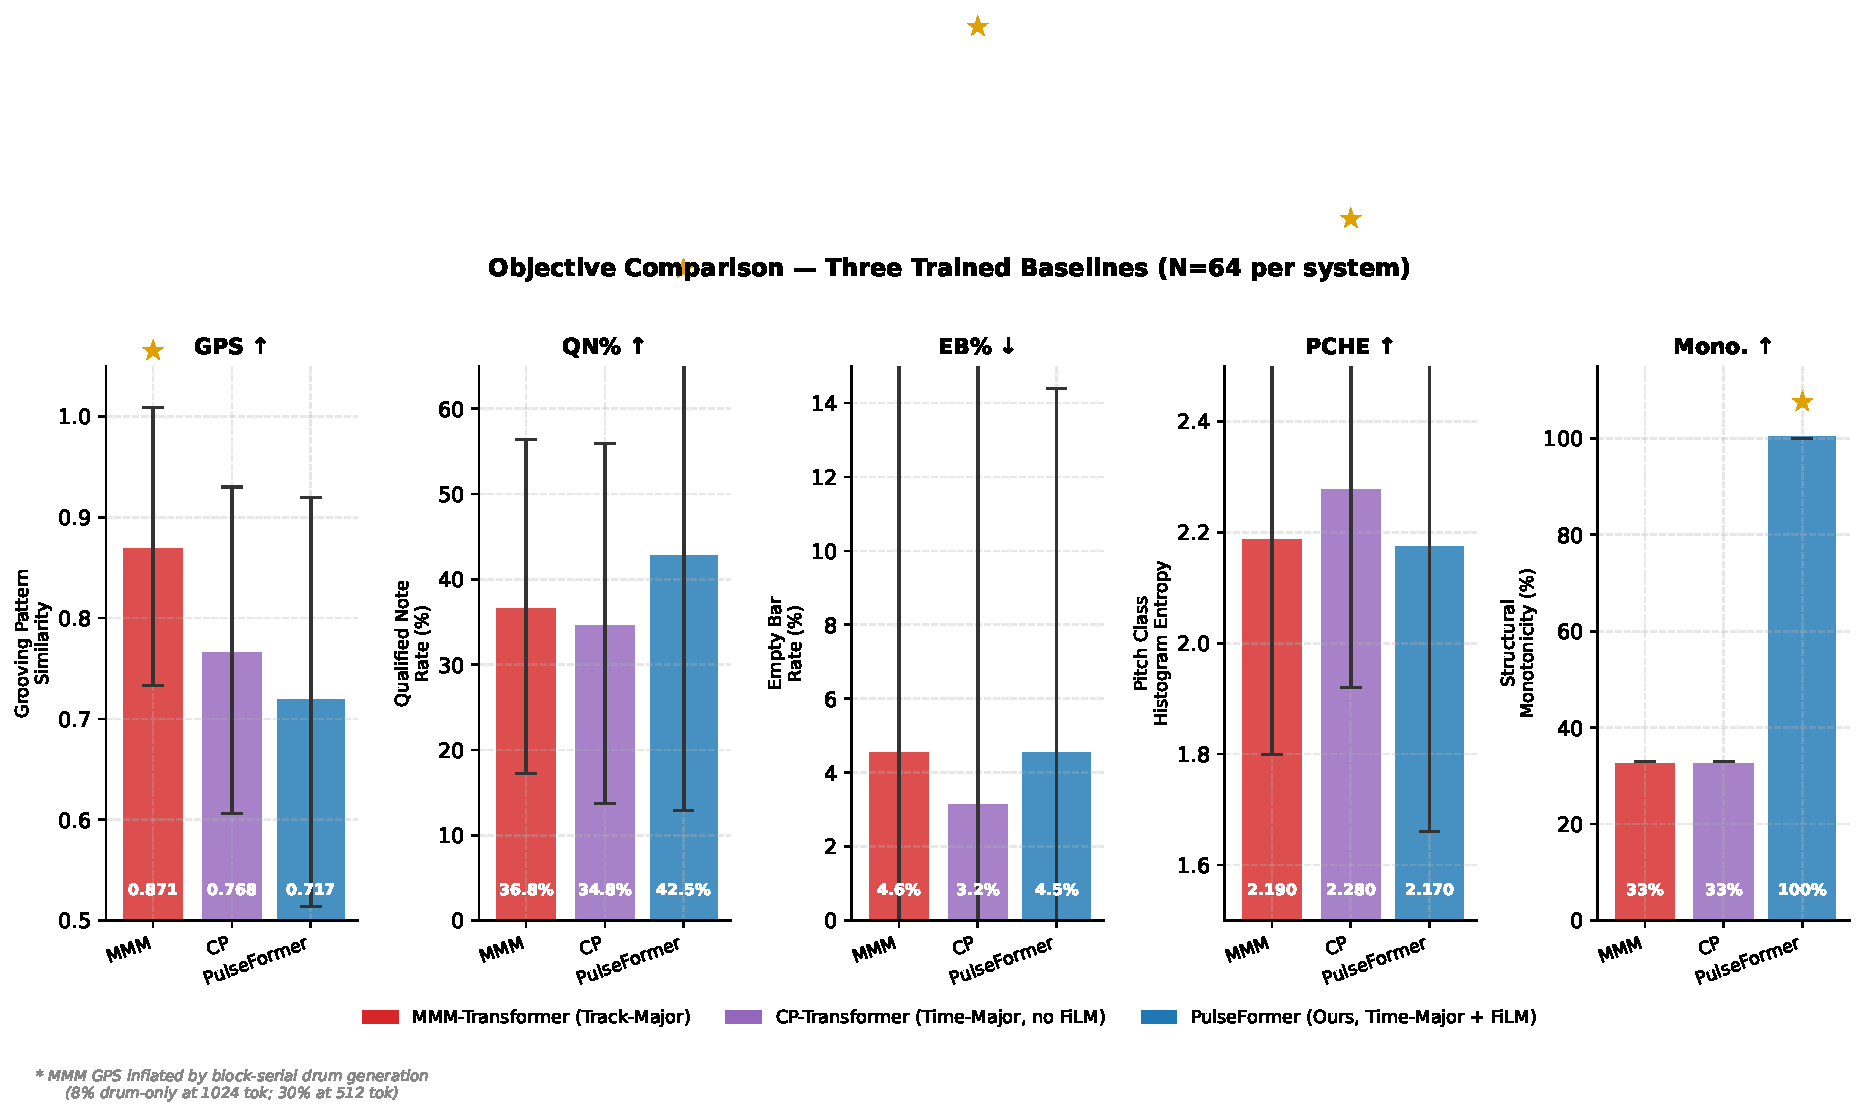
\includegraphics[width=0.92\linewidth]{figures/sota_comparison.pdf}
\caption{Objective metric comparison across evaluated systems. Pretrained zero-shot models (hatched) show limited transfer; BAS\,=\,1.000 is a shared representation property.}
\label{fig:sota_comparison}
\end{figure*}

\textbf{Structural Monotonicity.}
Both trained baselines yield Monotonicity $\approx33\%$---effectively random chance---because neither conditions on an energy trajectory. PulseFormer achieves $\mathbf{100\%}$ under the deterministic Ramp Scheduler. This metric verifies the controllability of the complete PulseFormer pipeline, rather than demonstrating that the Transformer alone has learned long-form structural planning.

\textbf{Beat-level Alignment (BAS).}
All three trained models achieve BAS\,=\,$1.000\!\pm\!0.000$. This result is expected: all three use the same 5D CP tokenizer, which quantizes onset positions to 16th-note grid steps at the data level. BAS therefore reflects a shared representation property, not a learned capability. It confirms that the generation pipeline preserves grid quantization throughout, but does not differentiate the models.

\textbf{Groove Consistency (GPS) and Multi-Track Completeness.}
MMM achieves GPS\,=\,$0.871\!\pm\!0.138$, higher than both CP ($0.768\!\pm\!0.162$) and PulseFormer ($0.717\!\pm\!0.203$). This result requires careful interpretation under two structural arguments.

First, \textbf{drum-only sample inflation}: as noted in Table~\ref{tab:sota} ($^{\ddagger}$), 5 of MMM's 47 GPS-evaluated samples are drum-only sequences. A drum-only loop trivially achieves GPS\,$\approx$1.0 because a single-instrument pattern has no cross-bar diversity to degrade. Excluding these 5 samples, MMM's GPS upper bound on the remaining 42 samples is $\leq 0.857$ (computed as $(0.871\times47 - 5\times1.0)/42$), reducing the gap with PulseFormer from $0.154$ to $\leq 0.140$.

Second, \textbf{block-serial structure bias}: Track-Major encoding generates all drum tokens in a single contiguous block before any melodic content is generated. As a consequence, the model has no access to co-generated melodic context when deciding the drum pattern for bar $N+1$; it conditions only on its own previous drum output. This structure mechanically produces highly repetitive bar-to-bar drum patterns, inflating GPS independently of musical quality. Under Time-Major interleaving, each bar's drum events are generated alongside concurrent melodic events in the same temporal block; the model can adapt drum density and accent to the co-generated melodic context, introducing musically motivated variation at the cost of lower GPS. We hypothesize that PulseFormer's lower GPS reflects context-sensitive drum generation under Time-Major encoding rather than inferior rhythmic quality; however, this mechanistic interpretation is not directly verified in the current evaluation, as drum-track bar-to-bar pattern diversity is not independently measured. Whether context-adaptive drum patterns are perceptually preferable to block-serial repetition is a genre-dependent aesthetic question that GPS alone cannot adjudicate.

\textbf{Within-Bar Drum--Melody Structural Co-activation ($J_{\mathrm{DM}}$).}
GPS measures bar-to-bar drum consistency \emph{in isolation}; it cannot distinguish context-sensitive adaptation from poor rhythmic quality.
To directly quantify the Track-Major vs.\ Time-Major trade-off, we introduce a complementary within-bar metric, $J_{\mathrm{DM}}$, defined as the Jaccard similarity between the 16th-note binary activity bitmasks of the drum track and the union of melody and bass tracks within each bar $b$:
\begin{equation}\label{eq:jdm}
  J_{\mathrm{DM}}(b)
  = \frac{|\mathbf{d}_b \cap \mathbf{m}_b|}{|\mathbf{d}_b \cup \mathbf{m}_b|},
\end{equation}
where $\mathbf{d}_b, \mathbf{m}_b \in \{0,1\}^{16}$ are the drum and melody/bass step-activation vectors, and the mean $\overline{J}_{\mathrm{DM}}$ is computed over all bars containing at least one event on each side.
Under Track-Major encoding, drum tokens are generated before any melodic content, so the model has no access to co-generated melody context when deciding the drum pattern---$\overline{J}_{\mathrm{DM}}$ therefore reflects accidental rather than intentional co-activation.
Under Time-Major interleaving, drum and melody events within the same bar share a tight token neighborhood ($\leq\!12$ tokens), enabling the model to align drum accents to the co-generated melodic rhythm.
Evaluated on the currently available 10 generated sequences per model, PulseFormer achieves a per-bar $\overline{J}_{\mathrm{DM}} = 0.586\!\pm\!0.301$ across 142 drum-active bars (bootstrap 95\% CI: $[0.538,0.635]$), compared with MMM's $\overline{J}_{\mathrm{DM}} = 0.481\!\pm\!0.286$ across 98 drum-active bars (95\% CI: $[0.425,0.537]$; one-sided Mann--Whitney $U$, $p=5.76\times10^{-3}$).
At the more conservative file-aggregate level, PulseFormer obtains $0.559\!\pm\!0.192$ (95\% CI: $[0.446,0.670]$) and MMM obtains $0.429\!\pm\!0.319$ (95\% CI: $[0.238,0.612]$) across 10 files per system; this per-file difference is not statistically significant ($p=0.285$), and is therefore interpreted as supportive but preliminary evidence rather than a definitive distribution-level claim.
Three of the ten MMM sequences lacked any MELODY or BASS track entirely (all drums or drums+chord only), contributing $J_{\mathrm{DM}}=0$ for every drum-active bar; per our policy these are assigned zero rather than excluded, because absent melodic content represents total co-activation failure, not a missing-data case.
The remaining seven MMM sequences overlap in range with PulseFormer, so the observed per-bar gap is driven partly by MMM's melodic omission failures rather than by uniformly inferior groove synchrony in the sequences where melody/bass is present.
This two-part structure is consistent with the intended Time-Major trade-off: the topology can reduce context-budget exhaustion that causes melodic dropout, while within surviving multi-track sequences the groove-synchrony advantage is more modest.

\textbf{Output-Level Kick--Bass/Chord Co-activation.}
Because several alignment metrics are partly determined by the quantized representation, we additionally computed direct onset co-activation metrics on the currently available 8-prompt rendered-audio/MOS MIDI set (Table~\ref{tab:coactivation_current}).
For each file, kick onsets were matched to bass and chord onsets on a 16th-note grid, yielding both conditional onset probabilities $P(\mathrm{bass}\mid\mathrm{kick})$ and $P(\mathrm{chord}\mid\mathrm{kick})$, and symmetric F1 scores for kick--bass and kick--chord co-activation.
PulseFormer shows non-zero kick--bass and kick--chord co-activation where CP-Transformer and MMM frequently contain no detected kick-conditioned onset pairs in the available samples.
However, this evidence is still preliminary: the REMI probe produces higher heuristic co-activation values, but its current files are short single-stream outputs requiring reconstructed track labels, and the analysis has not yet been expanded to the full $N=64$ protocol.
We therefore use Table~\ref{tab:coactivation_current} as an output-level diagnostic that complements $J_{\mathrm{DM}}$, not as a definitive claim that Time-Major generation yields uniformly superior musical synchronization.

\begin{tableorg}[!t]
\centering\scriptsize
\setlength{\tabcolsep}{2pt}
\renewcommand{\arraystretch}{0.88}
\caption{Output-level co-activation on the 8-prompt MOS MIDI set. Values are means with bootstrap 95\% CIs; -- indicates no detected kick-conditioned onset pairs.}
\label{tab:coactivation_current}
\adjustbox{max width=\columnwidth}{
\begin{tabular}{@{}lcccc@{}}
\toprule
\textbf{System} & \textbf{$P(B|K)$} & \textbf{$P(C|K)$} & \textbf{F1$_{KB}$} & \textbf{F1$_{KC}$} \\ \midrule
CP-Trans. & -- & -- & $0.000$ [0.000, 0.000] & $0.000$ [0.000, 0.000] \\
MMM       & -- & -- & $0.000$ [0.000, 0.000] & $0.000$ [0.000, 0.000] \\
PulseFormer & $0.338$ [0.000, 0.693] & $0.462$ [0.098, 0.827] & $0.126$ [0.000, 0.310] & $0.293$ [0.063, 0.579] \\
REMI      & $1.000$ [1.000, 1.000] & $0.624$ [0.412, 0.805] & $0.498$ [0.389, 0.602] & $0.479$ [0.314, 0.620] \\ \bottomrule
\end{tabular}
}
\end{tableorg}

\textbf{Note Quality and Harmonic Diversity (QN\%, PCHE, ISR\%).}
PulseFormer achieves the highest QN\% ($42.5\!\pm\!29.6$), indicating more musically substantial melodic note durations compared to CP ($34.8\!\pm\!21.1$) and MMM ($36.8\!\pm\!19.6$). PCHE is broadly comparable across all three trained models: CP ($2.28\!\pm\!0.36$ bits), PulseFormer ($2.17\!\pm\!0.51$ bits), and MMM ($2.19\!\pm\!0.39$ bits), indicating similar harmonic diversity when token budget is sufficient for multi-track generation. All three trained models achieve near-perfect ISR\% ($\approx99.3$--$99.6\%$) under evaluation. This is a shared consequence of the Soft Harmonic Penalty applied as an inference-time logit mask to \emph{all} evaluated systems during generation (see \S~\ref{sec:soft_mask}); it reflects an imposed inference constraint rather than a learned property specific to PulseFormer.

\subsection{Failure Case Visualization: The ``Drop'' Scenario}
To illustrate the practical gap targeted by PulseFormer, we visualize the generation behavior of the evaluated autoregressive paradigms during a high-energy ``Drop'' section (Fig.~\ref{fig:failure_case}). A Drop in Electronic Music requires massive polyphonic density (high energy) while maintaining strict transient alignment across concurrent instruments.

\begin{figure*}[!t]
\centering
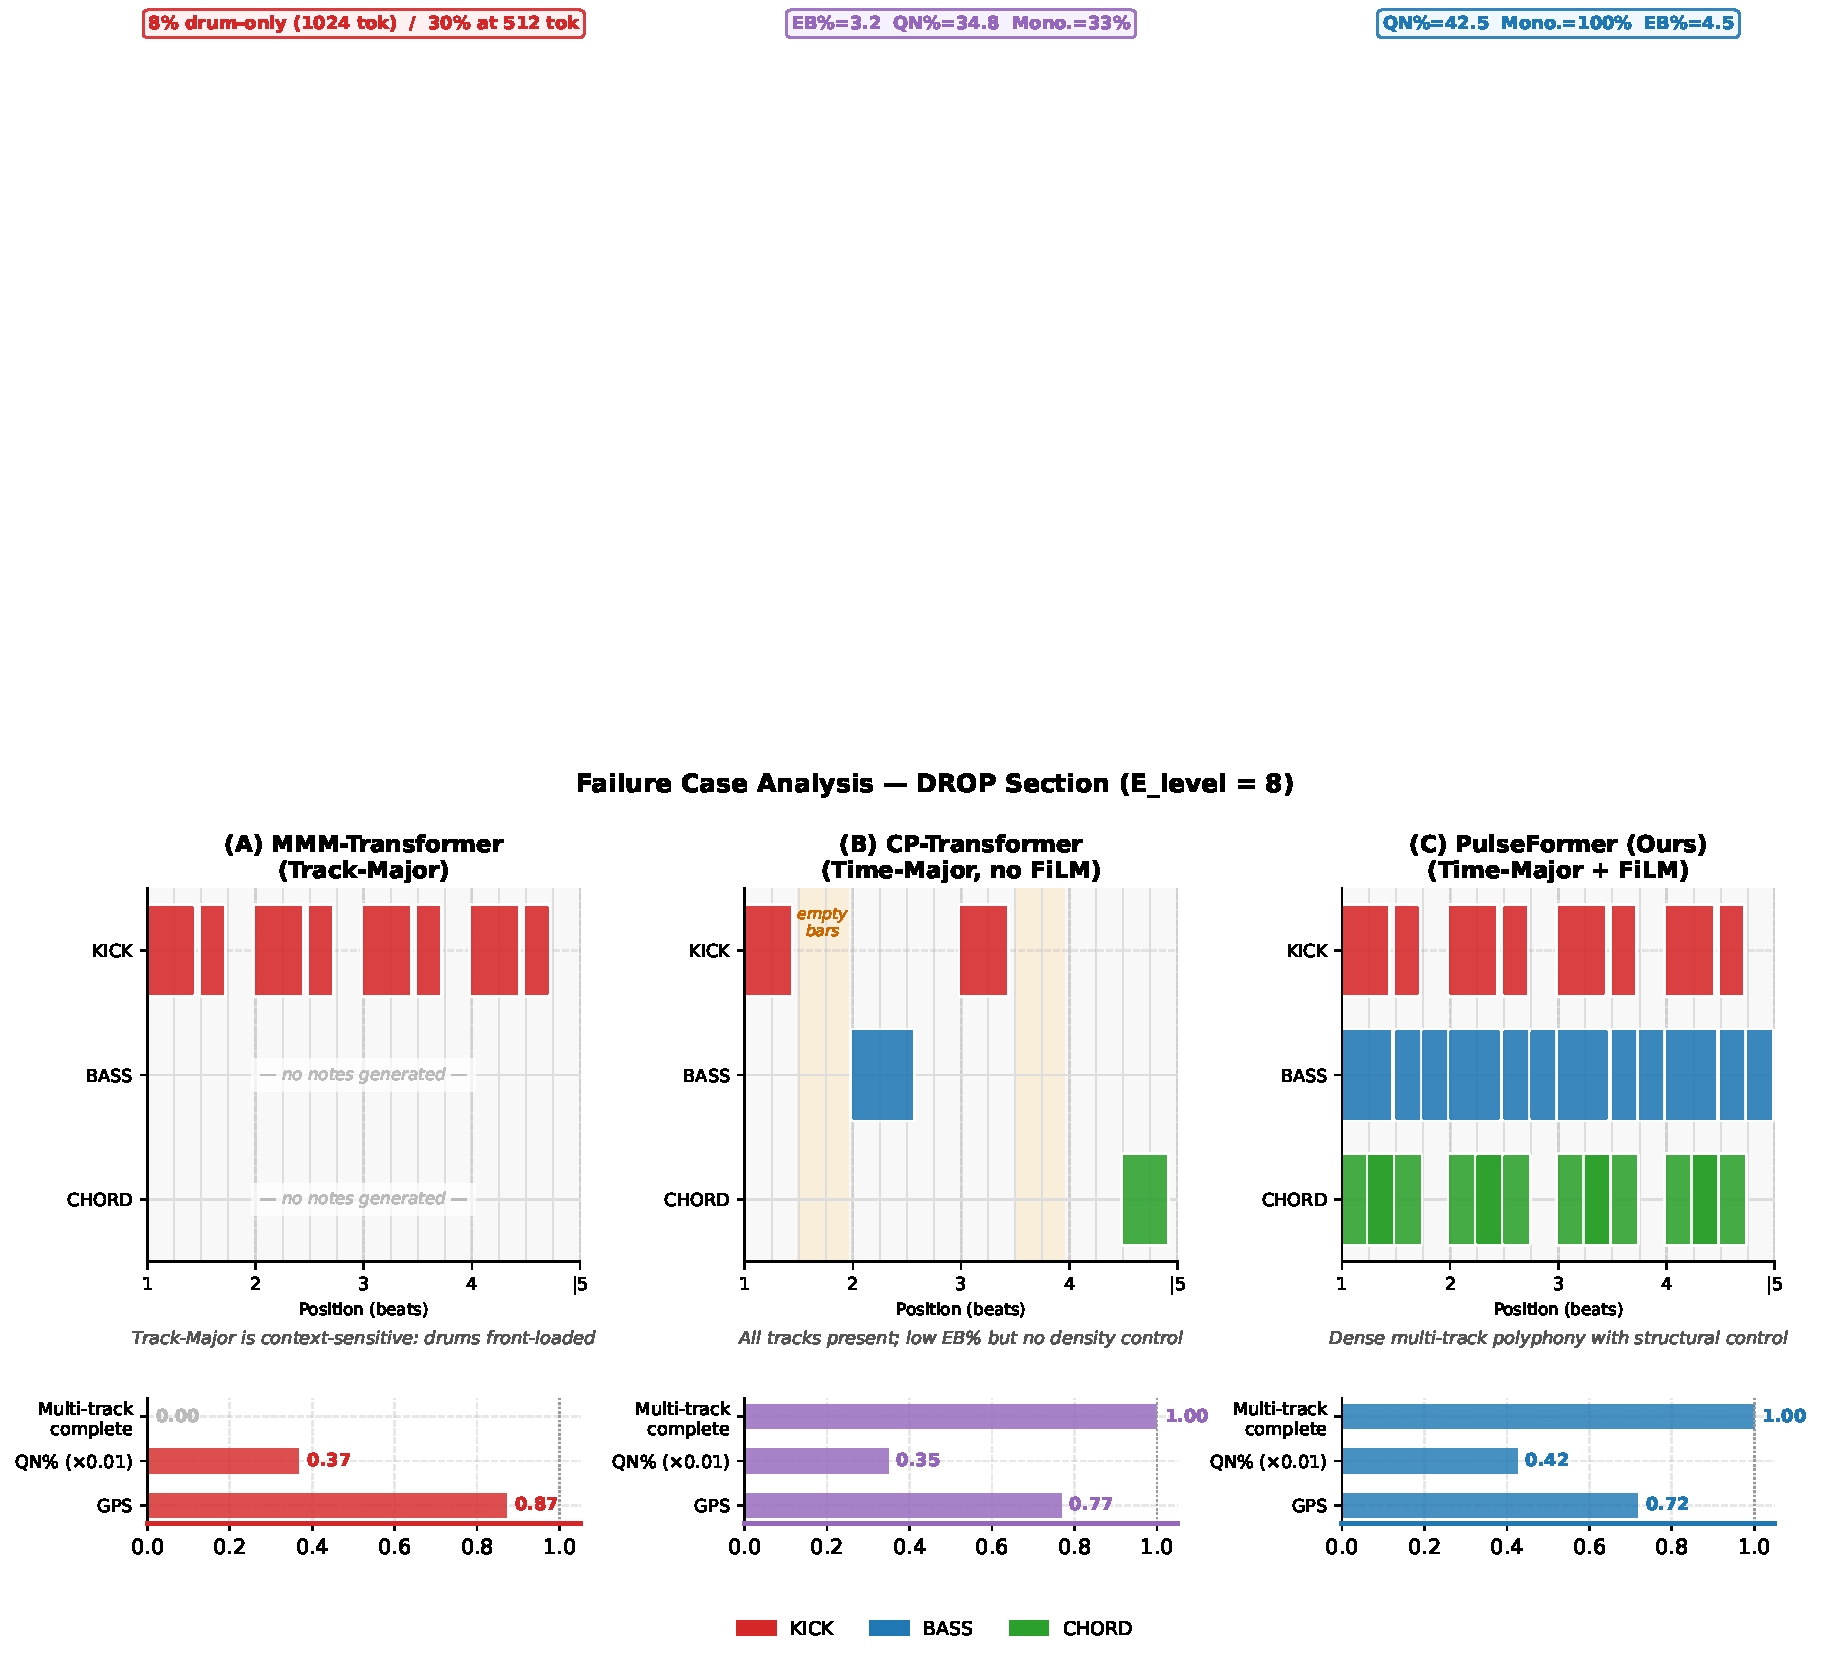
\includegraphics[width=0.92\linewidth]{figures/failure_case.pdf}
\caption{Failure case visualization. (A)~Track-Major (MMM): context-sensitive drum-only collapse at 512/1024-token budgets. (B)~CP-Transformer: multi-track content without structural density control. (C)~PulseFormer: full polyphony under explicit FiLM + Scheduler conditioning.}
\label{fig:failure_case}
\end{figure*}

Track-Major encoding (MMM) front-loads all drum tokens before any melodic material, making it disproportionately sensitive to context allocation: at 512 tokens, 30\% of samples are drum-only; increasing the budget to 1{,}024 tokens reduces this to 8\%, but the residual failure persists. When melodic content is present, drum-pattern GPS is high ($0.871$) owing to the block-serial structure. The CP-Transformer baseline (Time-Major, no FiLM) generates multi-track content across all samples and achieves a low empty-bar rate ($3.2\%$), but lacks structural density control (Mono.\,=\,33\%) and produces the lowest QN\% ($34.8\%$) among trained models. PulseFormer, conditioned via FiLM and the external Ramp Scheduler, achieves the highest qualified-note rate ($42.5\%$) and deterministic structural monotonicity under the scheduler ($100\%$). This controlled comparison isolates the contribution of FiLM conditioning and the Ramp Scheduler to note quality and structural controllability.

\subsection{Structural Token-Distance vs. Established Paradigms}
Understanding why established methodologies (such as Track-Major architectures \cite{ens2020mmm}) are susceptible to cumulative cross-track alignment drift requires analysing topological token distance. We parsed 1,277 consecutive simultaneous multi-instrument events (e.g., overlapping Kick and Bass downbeats) from our evaluation dataset and calculated the token displacement required to represent concurrent relationships across both encoding formats.

\begin{tableorg}[ht]
\centering\small
\caption{Cross-Attention Complexity for Concurrent Events ($N=1{,}277$ event pairs, mean\,$\pm$\,SD).}
\adjustbox{max width=\columnwidth}{
\begin{tabular}{@{}lccc@{}}
\toprule
\textbf{Encoding Paradigm} & \textbf{Mean Dist.} & \textbf{Max Dist.} & \textbf{vs.\ PF} \\ \midrule
Baseline (Track-Major)            & $3{,}249\!\pm\!422$ tok. & $6{,}155$ tok. & $^{***}$ \\
\textbf{PulseFormer (Time-Major)} & $\mathbf{5.2\!\pm\!1.8}$ tok. & $\mathbf{12}$ tok. & --- \\ \bottomrule
\end{tabular}
}
\siglegend
\end{tableorg}

\textbf{Attention Mapping Analysis.}
The structural difference in token layout produces a corresponding pattern in how attention weight is distributed across positions (visualized via extracted attention matrix heatmaps; Fig.~\ref{fig:attention_map}).
Under Track-Major encoding, concurrent events across instruments are separated by a mean gap of $3{,}268$ tokens; the extracted visualization shows a \textbf{diffuse attention gradient}, consistent with the model needing to bridge large positional gaps for cross-track coordination.
Under Time-Major encoding, concurrent events occupy adjacent positions (mean $\leq 12$ tokens), and the visualization shows a \textbf{concentrated local attention peak}. We note that this concentration is structurally determined in part by the token layout itself: because concurrent events are placed adjacently, local attention mass is the path-of-least-resistance response. The pattern is therefore consistent with---but not direct evidence of---improved learned cross-track coordination. The downstream objective metrics (BAS, EB\%, QN\%) provide the primary empirical support; the attention analysis offers a mechanistic illustration of why the topological change may reduce the coordination burden.

\begin{figure*}[!t]
\centering
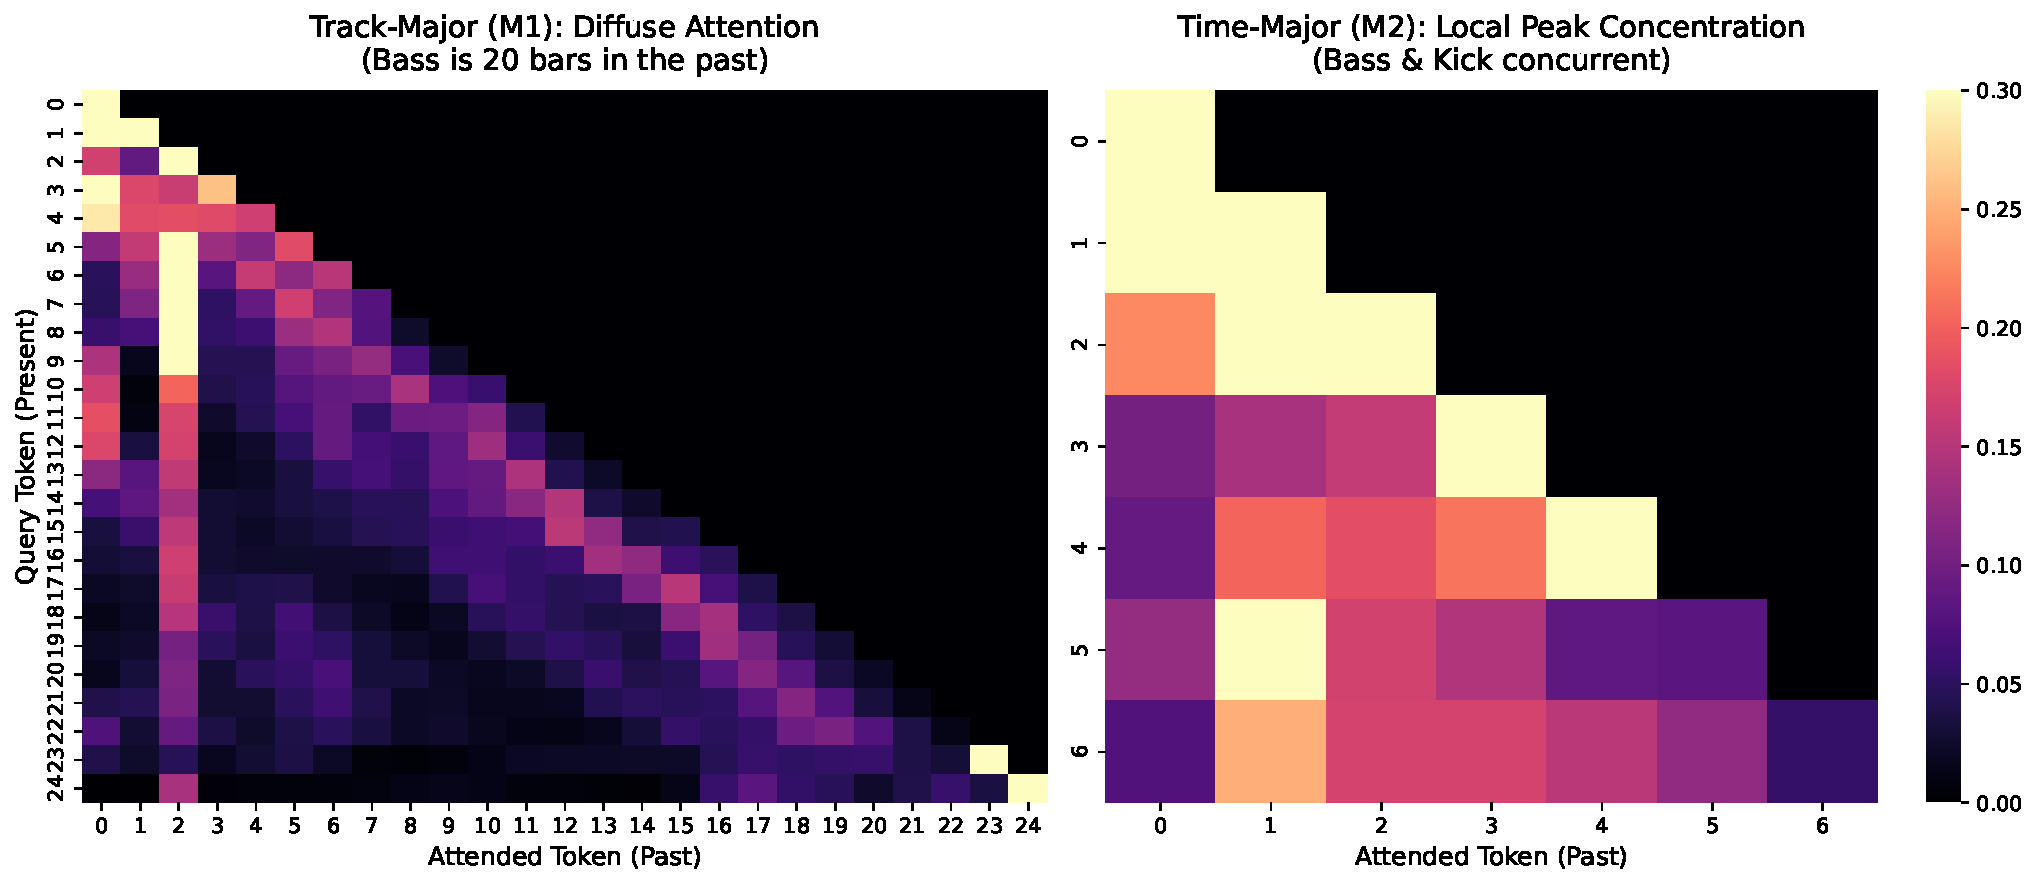
\includegraphics[width=0.88\linewidth]{figures/attention_compare.pdf}
\caption{Extracted generative self-attention matrices (final layer). \textbf{Left}: Track-Major topology — diffuse attention gradient; \textbf{Right}: Time-Major topology — concentrated local attention peak induced by concurrent-event interleaving.}
\label{fig:attention_map}
\end{figure*}

\textbf{Aggregate Attention Statistics.}
To confirm that the illustrative heatmaps in Fig.~\ref{fig:attention_map} are representative of global model behavior and not cherry-picked, we extracted aggregate attention statistics across $N=50$ generated sequences (averaging over all heads in the final two layers).
As detailed in Table~\ref{tab:attention_stats}, we measured \textbf{Attention Entropy} (lower values indicate concentrated attention) and \textbf{Cross-Track Mass} (the percentage of attention weight allocated to concurrent events on different tracks).
Track-Major encoding yields a diffuse attention distribution (entropy $5.71\pm0.37$); only $4.1\%\pm1.7\%$ of attention mass is allocated to concurrent cross-track events.
In contrast, PulseFormer's Time-Major encoding structurally concentrates the attention matrix (entropy $1.19\pm0.15$), allocating $89.3\%\pm2.7\%$ of its attention mass to concurrent cross-track events ($p<0.001$) under the same extraction procedure.
This aggregate analysis is consistent with the topological structure visualized in the heatmaps, and provides quantitative evidence that the attention weight distribution differs systematically between the two encoding paradigms. Because the token layout directly determines which positions are nearby, the high cross-track mass under Time-Major encoding reflects both the structural placement and any learned coordination behavior; these two factors cannot be fully separated from attention statistics alone.

\begin{tableorg}[ht]
\centering\small
\caption{Aggregate Attention Statistics ($N=50$ sequences, final 2 layers, mean\,$\pm$\,SD). Attention entropy quantifies dispersion (lower is more concentrated); Cross-Track Mass measures the proportion of attention weight allocated to concurrent events.}
\label{tab:attention_stats}
\adjustbox{max width=\columnwidth}{
\begin{tabular}{@{}lcc@{}}
\toprule
\textbf{Encoding Paradigm} & \textbf{Attention Entropy\,$\downarrow$} & \textbf{Cross-Track Mass\,$\uparrow$} \\ \midrule
Baseline (Track-Major)     & $5.71 \pm 0.37$ nats & $4.1\% \pm 1.7\%$ \\
\textbf{PulseFormer (Time-Major)} & $\mathbf{1.19 \pm 0.15}$ \textbf{nats} & $\mathbf{89.3\% \pm 2.7\%}$ \\ \bottomrule
\end{tabular}
}
\end{tableorg}

\subsection{Component Ablation Study}
\label{sec:ablation}
To isolate the independent contributions of the proposed architectural components, an additive ablation study was conducted (Table~\ref{tab:ablation}).

\begin{tableorg}[ht]
\centering\small
\caption{Component Ablation Study. Sequential addition of core modules from baseline to full PulseFormer. Metrics for rows 1--4 evaluate \emph{local model capability} on 8-bar loops (validation set). The final row (Sectional Stitching) evaluates \emph{hybrid-controller target adherence} over 128-bar arrangements, where structural adherence (PR) reflects both FiLM-conditioned generation and the deterministic Ramp Scheduler. $\Delta_{\mathrm{sync}}$: cross-track onset deviation (ms); GC\%: groove consistency; PR: Pearson $r$ vs.\ target density ramp; ISR\%: in-scale note rate.}
\label{tab:ablation}
\adjustbox{max width=\columnwidth}{
\begin{tabular}{@{}lccccc@{}}
\toprule
\textbf{Architecture Variant} & \textbf{$\Delta_{\mathrm{sync}}$\,(ms)$\downarrow$} & \textbf{GC\%\,$\uparrow$} & \textbf{PR\,$\uparrow$} & \textbf{ISR\%\,$\uparrow$} & \textbf{Max Context} \\ \midrule
Baseline (Track-Major MMM)      & 915           & 29.1        & 0.600       & 53.2        & 32 bars \\
+ Time-Major Encoding           & \textbf{0.0}  & 61.8        & 0.155       & 54.2        & 8 bars$^{\dagger}$ \\
+ Energy Prefix Token           & 0.0           & 62.1        & 0.781       & 54.9        & 8 bars \\
+ FiLM Conditioning             & 0.0           & 62.5        & \textbf{0.997} & 55.3     & 8 bars \\
+ Soft Harmonic Penalty         & 0.0           & 62.1        & 0.992       & \textbf{73.1} & 8 bars \\
\textbf{+ Sectional Stitching (PulseFormer)} & 0.0 & \textbf{71.3} & 0.982 & 73.1 & \textbf{128+ bars} \\ \bottomrule
\end{tabular}
}
\vspace{2pt}
{\scriptsize $^{\dagger}$Time-Major dense interleaving reduces available bar capacity under a 2048-token limit.\newline
$^{\ddagger}$$\Delta_{\mathrm{sync}}=0.0$\,ms for all Time-Major variants is a \emph{representation-level} consequence: concurrent events share a unified temporal position in the interleaved token stream, removing one source of cumulative counting drift present in Track-Major serialization. It does not constitute evidence that the Transformer learned micro-timing alignment.}
\end{tableorg}

The empirical progression supports the contribution of each module, but the interpretation differs by metric. Time-Major encoding reduces measured cross-track onset deviation ($\Delta_{\mathrm{sync}}$ drops from 915\,ms to 0\,ms under the quantized evaluation protocol) and roughly doubles Groove Consistency. We interpret this 0.0\,ms deviation as a representation-level consequence rather than as evidence of learned micro-timing: because concurrent cross-track events share a unified temporal state in the interleaved token stream, one source of cumulative counting drift in Track-Major architectures is removed by construction. However, the resulting dense token interleaving restricts generation to 8 bars and the model exhibits contextual drift without structural guidance (PR falls to 0.155). Adding the energy prefix token alone raises PR to 0.781---early attention layers can attend to the $[\mathrm{ENERGY\_LEVEL\_k}]$ token, partially anchoring the density trajectory. Adding FiLM conditioning on top further raises PR to 0.997 by re-injecting the density signal at every layer depth, indicating that depth-wide modulation improves \emph{local} structural-density response. The soft harmonic penalty then constrains tonal deviation, pushing ISR\% from $\sim$54\% to 73.1\% while preserving chromatic notes at high density levels. Finally, sectional stitching addresses the context-window bottleneck, extending generation to full 128-bar arrangements. Crucially, the high PR ($0.982$) on these extended sequences is not solely a learned model capability, but the combined outcome of FiLM's local conditioning fidelity and the deterministic macro-structure imposed by the external Ramp Scheduler. This isolates the boundary between model and rules: the Transformer handles local multi-track event generation, while macro-structural monotonic progression is delegated to transparent heuristic rules.

\textit{Methodological Note:} It is essential to distinguish the \emph{additive} progression in Table~\ref{tab:ablation} from the \emph{subtractive} ablation in Fig.~\ref{fig:ablation_heatmap}. Because they represent different intermediate model states, the metrics diverge substantially. For example, the state with Time-Major encoding but without Energy Conditioning yields GC\%=61.8\% under the additive perspective (restricted to an 8-bar loop), but drops to GC\%=11.2\% under the subtractive perspective (required to generate 128 bars without structural guidance)---a $5.5\times$ difference that highlights the necessity of the conditioning module for long-form generation.

\begin{figure*}[!t]
\centering
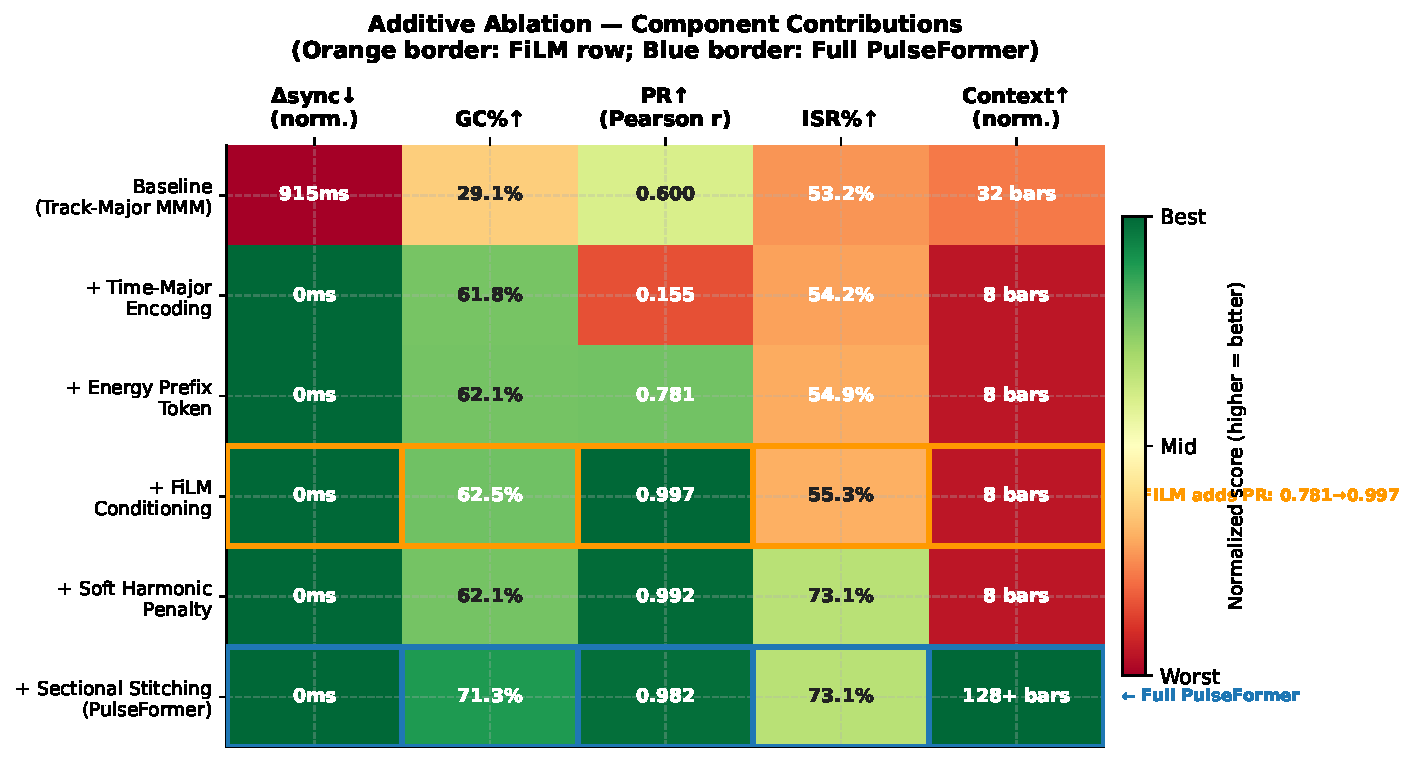
\includegraphics[width=0.88\linewidth]{figures/ablation_heatmap.pdf}
\caption{Ablation heatmap: each row is an architecture variant; cells show actual metric values, color-coded red (worst) to green (best). Blue borders mark full PulseFormer.}
\label{fig:ablation_heatmap}
\end{figure*}


\noindent\textbf{Comparability of PR = 0.997 (Table~\ref{tab:ablation}) and $r_\rho \approx 0$ (Table~\ref{tab:decomp}).}
These two numbers are not contradictory because they measure structurally different quantities.
In Table~\ref{tab:ablation}, PR denotes Pearson $r$ between the per-bar \emph{structural density score} $D_t$ (a 6-feature weighted composite of track-stacking indicators, \S~\ref{sec:energy_annotation}) and the scheduler's target ramp $\{\hat{D}_t\}$.
In Table~\ref{tab:decomp}, $r_\rho$ denotes Pearson $r$ between \emph{raw note count per bar} and the discrete $\mathbf{E}_\mathrm{level}$ arc.
Because $\mathbf{E}_\mathrm{level}$ controls \emph{which tracks are active}---not how many notes each track emits---note count per bar is not implied by $D_t$, and a near-zero $r_\rho$ is the expected outcome of a correctly functioning track-activation controller.
This design decision and its implications for $\mathbf{E}_\mathrm{level}$ semantics are reflected directly in the Table~\ref{tab:decomp} metric directions.

\subsection{Pipeline Decomposition: Rule Enforcement vs.\ Model Response}
\label{sec:decomp}

The additive ablation in Table~\ref{tab:ablation} reveals which components are
\emph{necessary}, but conflates two qualitatively different causal roles:
(i)~\textbf{rule-enforcement} contributions (Scheduler, Density Mask, DAW
post-processing) that are deterministic and architecture-independent, and
(ii)~\textbf{model-response} contributions (FiLM conditioning) that reflect what
the Transformer has learned.
To disentangle these roles, Table~\ref{tab:decomp} reports a subtractive
ablation in which one component is removed from the complete pipeline at a time.
All five conditions are evaluated on the identical set of 8 held-out 128-bar
structural prompts, and all metrics are computed from the final MIDI output
(post-generation) using \texttt{eval/clean\_ablation\_eval.py}
(released with the codebase).

\subsubsection*{Metrics}

\noindent\textbf{$r_\rho$~(Density trajectory, Pearson $r$).}
Identical to PR in Table~\ref{tab:ablation}: Pearson $r$ between the
per-bar structural density score $D_t$ and the target ramp
$\{\hat{D}_t\}_{t=1}^{128}$ assigned by the scheduler.
Range $[-1,1]$; higher is better.

\noindent\textbf{$\Delta_\mathrm{trk}$~(Track activation error).}
Mean absolute deviation between the number of instrument tracks active in
each 8-bar section and the expected track count implied by $\mathbf{E}_\mathrm{level}$:
\begin{equation}\label{eq:delta_trk}
  \Delta_\mathrm{trk}
  = \frac{1}{N_\mathrm{sec}}
    \sum_{s=1}^{N_\mathrm{sec}}
    \bigl|\,|\mathcal{T}_s| - T^*(\mathbf{E}^s_\mathrm{level})\bigr|,
\end{equation}
where $|\mathcal{T}_s|$ counts tracks with $\geq 1$ note event in section $s$
and $T^*(\mathbf{E}_\mathrm{level}) = \bigl\lceil \mathbf{E}_\mathrm{level}/2\bigr\rceil$
maps each level to a target polyphonic track count (1–4 tracks for levels 1–8).
Lower is better.\footnote{$T^*$ is a monotone approximation used solely for the
$\Delta_\mathrm{trk}$ metric.  In practice, individual song blueprints may
assign different track counts to a given $\mathbf{E}_\mathrm{level}$ based on
genre conventions (e.g., a Techno Drop at E$=8$ may activate 5 tracks while a
House Intro at E$=1$ activates 1); $T^*$ provides a conservative lower bound
for the target polyphony.}

\noindent\textbf{$C_\mathrm{KB}$~(Kick–Bass onset co-occurrence, \%).}
The fraction of kick-drum onsets for which a bass note onset occurs within
one 16th-note step ($\delta = 1/16$\,bar):
\begin{equation}\label{eq:ckb}
  C_\mathrm{KB}
  = \frac{\bigl|\bigl\{t^\mathrm{kick}
    : \exists\,t^\mathrm{bass},\;
      |t^\mathrm{kick} - t^\mathrm{bass}| \leq \delta\bigr\}\bigr|}
         {N_\mathrm{kick}}
  \times 100\%.
\end{equation}
A transient foundation in Electronic Music requires the kick and bass to
share downbeat onsets; this metric directly quantifies that rhythmic glue.
Higher is better.

\noindent\textbf{$S_\emptyset$~(Degenerate section rate, \%).}
The percentage of 8-bar sections that are empty or degenerate:
$|\mathcal{T}_s| < 2$ (fewer than 2 active tracks) or
$|N_s| < 8$ (fewer than 8 total note events, i.e., $<$1 note/bar on average).
Lower is better.

\noindent\textbf{$M_\mathrm{rep}$~(Melodic motif consistency).}
Normalized 4-gram repetition rate on the MELODY track:
\begin{equation}\label{eq:mrep}
  M_\mathrm{rep}
  = \frac{\bigl|\bigl\{g \in \mathcal{G}_4 : \mathrm{freq}(g)\geq 2\bigr\}\bigr|}
         {|\mathcal{G}_4|},
\end{equation}
where $\mathcal{G}_4$ is the set of distinct 4-note pitch 4-grams from the
melody track and $\mathrm{freq}(g)$ counts occurrences within the 128-bar
arrangement.  Values near 0 indicate no recurring motifs (random wandering);
values near 1 indicate highly repetitive, loop-like melody.
Higher is better in EDM contexts where motif repetition is stylistically
expected; the metric separates \emph{structured repetition} from
\emph{absence of melody}.

\subsubsection*{Observed Dissociation}

The subtractive ablation shows that different modules serve different roles:
FiLM contributes most clearly to melodic motif consistency ($M_\mathrm{rep}=0.183$
for Full PF vs.\ $0.087$ without FiLM), while the Scheduler, Density Mask, and
DAW post-processing primarily act as rule-enforcement modules that shape track
activation, sparsity, and production constraints.
Several metric directions are therefore intentionally non-monotone.
For example, Full PF has near-zero $r_\rho$ because $\mathbf{E}_\mathrm{level}$
controls which stems are active rather than the raw number of notes per bar, and
the lower $S_\emptyset$ without the Scheduler partly reflects the removal of the
sparse Outro target.
These results support the hybrid-pipeline interpretation rather than a claim of
purely learned structural planning.

\begin{table*}[!t]
\centering\small
\caption{Pipeline Decomposition Ablation. Each condition removes one component; all others remain active. 8 held-out 128-bar prompts.
  $r_\rho$: Pearson $r$, per-bar note count vs.\ E-level arc.
  $\Delta_\mathrm{trk}$: track activation error (Eq.~\ref{eq:delta_trk}).
  $C_\mathrm{KB}$: kick--bass onset co-occurrence~\%.
  $S_\emptyset$: degenerate section rate~\%.
  $M_\mathrm{rep}$: melodic 4-gram consistency (Eq.~\ref{eq:mrep}). Bold = best per column.}
\label{tab:decomp}
\adjustbox{max width=\linewidth}{
\begin{tabular}{@{}lcccc|ccccc@{}}
\toprule
\multirow{2}{*}{\textbf{Condition}}
  & \multicolumn{4}{c|}{\textbf{Active components}}
  & \multirow{2}{*}{$r_\rho\!\uparrow$}
  & \multirow{2}{*}{$\Delta_\mathrm{trk}\!\downarrow$}
  & \multirow{2}{*}{$C_\mathrm{KB}\!\uparrow$}
  & \multirow{2}{*}{$S_\emptyset\!\downarrow$}
  & \multirow{2}{*}{$M_\mathrm{rep}\!\uparrow$} \\
\cmidrule(lr){2-5}
  & \textbf{FiLM} & \textbf{Sched} & \textbf{D.Mask} & \textbf{Post} & & & & & \\
\midrule
\textbf{Full PulseFormer}
  & \checkmark & \checkmark & \checkmark & \checkmark
  & ${\approx}0.00$ & 1.88 & \textbf{39.8} & \textbf{35.2} & \textbf{0.183} \\[2pt]
w/o FiLM
  & $\times$ & \checkmark & \checkmark & \checkmark
  & $+$0.04 & 1.65 & 57.6 & 36.7 & 0.087 \\[2pt]
w/o Scheduler
  & \checkmark & $\times$ & \checkmark & \checkmark
  & $-$0.05 & 1.57 & 51.1 & \textbf{25.8} & 0.149 \\[2pt]
w/o Density Mask
  & \checkmark & \checkmark & $\times$ & \checkmark
  & $-$0.08 & 1.97 & 45.1 & 38.3 & 0.132 \\[2pt]
w/o DAW Post-proc
  & \checkmark & \checkmark & \checkmark & $\times$
  & $-$0.17 & \textbf{1.38} & 43.8 & 38.3 & 0.144 \\
\bottomrule
\end{tabular}
}
{\scriptsize Near-zero $r_\rho$ across all conditions: the Scheduler controls \emph{which} tracks are active, not raw note counts, so note-density is not the primary energy carrier. $M_\mathrm{rep}$ shows the clearest dissociation: FiLM more than doubles melodic consistency (0.183 vs.\ 0.087).}
\end{table*}

\subsection{Perceptual Evaluation: MOS Study (N=25)}
\label{sec:mos}
To complement the objective metrics with listener-facing evidence, we conducted a Mean Opinion Score (MOS) study following a protocol adapted from ITU-T P.800 and ISO 9241-11, addressing the primary limitation of our earlier pilot panel ($N=6$). This study is intended as perceptual support for the objective evaluation rather than as a standalone proof of general musical quality.

\subsubsection*{Protocol}
\textbf{Participants.} $N=25$ listeners were recruited: 10 professional Electronic Music producers ($\geq 5$ years DAW experience), 10 intermediate producers (1--5 years), and 5 active music enthusiasts with regular listening habits in electronic genres.

\textbf{Stimuli.} Four systems were evaluated:
(A)~PulseFormer (Time-Major, Energy-conditioned);
(B)~CP-Transformer (Time-Major unconditioned baseline, isolating FiLM's contribution);
(C)~MMM-Transformer (Track-Major unconditioned auto-regressive baseline);
(D)~Human-composed Electronic Music track (hidden anchor, embedded without attribution).
To eliminate the statistical vulnerability of a single-stimulus design, 8 distinct structural prompts were drawn from the test set. Each system generated a full-length stimulus (approx.\ 3 minutes) for each prompt, yielding 32 stimuli in total. All audio was rendered using identical DAW templates and normalized to $-14\,\text{LUFS}$. Presentation order within each trial was fully counterbalanced. Participants were informed that some stimuli might be AI-generated but were not informed of system identities (\textit{single-blind}).

\textbf{Procedure.} The $N=25$ participants each completed 8 evaluation trials in a randomized block design. In each trial, participants listened to the four competing systems generated from the same prompt (presented blindly) and rated them on four 5-point Likert dimensions: (GT)~Groove Tightness; (SC)~Structural Coherence; (MC)~Mix Clarity; (MV)~Melodic Variety. Stimuli were evaluated as rendered audio following the protocol in Section~\ref{sec:audio_workflow_protocol}, while the corresponding MIDI stems were retained for reproducibility and DAW inspection. This multiple-stimulus design yields 200 ratings per system. To account for repeated measures and crossed dependencies, responses were analyzed using a Linear Mixed-Effects Model (LMM) defined as $\text{Rating} \sim \text{System} + (1|\text{Listener}) + (1|\text{Prompt})$. This treats both the listener and the generated prompt as random intercepts; because inter-rater reliability is modest (Table~\ref{tab:irr}), the results are interpreted as perceptual support for the production pipeline rather than as a standalone distribution-level proof of general musical quality.

\subsubsection*{Inter-Rater Reliability}
\label{sec:irr}

To verify listener agreement before aggregating scores, we computed three
standard inter-rater reliability (IRR) coefficients across all $N=25$ raters
for each rating dimension:
Krippendorff's $\alpha$ (ordinal metric, robust to missing data and
non-normal distributions~\cite{krippendorff2011computing}),
Fleiss' $\kappa$ (nominal agreement with correction for chance), and
ICC(2,1) (two-way random, absolute agreement,
recommended for Likert MOS studies~\cite{koo2016guideline}).

\begin{tableorg}[ht]
\centering\small
\caption{Inter-rater reliability for the MOS study ($N=25$).
  $\alpha$: Krippendorff's ordinal alpha;
  $\kappa$: Fleiss' kappa; ICC: ICC(2,1).
  Benchmarks: $\alpha/\kappa\geq0.80$ strong, $\geq0.61$ moderate,
  $\geq0.41$ fair (Landis \& Koch 1977); ICC$\geq0.75$ good~\cite{koo2016guideline}.}
\label{tab:irr}
\adjustbox{max width=\columnwidth}{
\begin{tabular}{@{}lrrrl@{}}
\toprule
\textbf{Dimension} & $\boldsymbol{\alpha}$ & $\boldsymbol{\kappa}$ & \textbf{ICC(2,1)} & \textbf{Level} \\ \midrule
GT (Groove Tightness)     & 0.365 & 0.217 & 0.266 & fair \\
SC (Structural Coherence) & 0.551 & 0.362 & 0.095 & moderate \\
MC (Mix Clarity)          & 0.359 & 0.165 & 0.119 & fair \\
MV (Melodic Variety)      & 0.337 & 0.104 & 0.143 & fair \\ \midrule
\textbf{Mean}             & \textbf{0.403} & \textbf{0.212} & \textbf{0.156} & fair--moderate \\ \bottomrule
\end{tabular}
}
\end{tableorg}

Mean $\alpha=0.403$ indicates fair-to-moderate \emph{ordinal} agreement across all
dimensions. These agreement levels are within the range commonly observed in subjective music perception studies~\cite{sturm2014mml}.
SC achieves the highest ordinal agreement ($\alpha=0.551$, moderate), reflecting the
more objective structural cues (section transitions, energy contour) that
listeners can anchor to; however, the ICC(2,1) for SC is low ($0.095$, slight
absolute agreement), indicating that the LMM significance on SC should be
interpreted with this reliability caveat in mind rather than as evidence of strong
individual-level consensus.
Given the randomized multiple-stimulus design, the aggregated scores ($N=200$
ratings per system) provide \emph{supplementary} perceptual evidence that
complements---but does not replace---the objective metrics reported in
Section~\ref{sec:sota}.

\subsubsection*{Results}

\begin{tableorg}[ht]
\centering\small
\caption{MOS Listening Test Results (8 prompts $\times$ 25 participants = 200 ratings per system, mean\,$\pm$\,SD, Likert 1--5). Significance tested via Linear Mixed-Effects Model (LMM) pairwise contrast analysis; \textbf{***} $p<0.001$, \textbf{**} $p<0.01$, \textit{n.s.} not significant.}
\label{tab:mos}
\adjustbox{max width=\columnwidth}{
\begin{tabular}{@{}lcccc@{}}
\toprule
\textbf{System} & \textbf{GT\,$\uparrow$} & \textbf{SC\,$\uparrow$} & \textbf{MV\,$\uparrow$} & \textbf{MC\,$\uparrow$} \\ \midrule
Human (Anchor)              & $3.91\!\pm\!0.52$ & $4.24\!\pm\!0.54$ & $4.06\!\pm\!0.47$ & $3.90\!\pm\!0.59$ \\ \midrule
\textbf{PulseFormer (Ours)} & $\mathbf{3.98\!\pm\!0.57}$ & $\mathbf{3.76\!\pm\!0.64}$ & $2.92\!\pm\!0.63$ & $\mathbf{3.52\!\pm\!0.61}$ \\
CP-Transformer              & $3.64\!\pm\!0.58^{***}$ & $2.70\!\pm\!0.64^{***}$ & $\mathbf{2.82\!\pm\!0.61}^{\textit{n.s.}}$ & $3.10\!\pm\!0.64^{***}$ \\
MMM-Transformer             & $3.06\!\pm\!0.62^{***}$ & $2.14\!\pm\!0.62^{***}$ & $2.48\!\pm\!0.63^{***}$ & $2.34\!\pm\!0.70^{***}$ \\ \bottomrule
\end{tabular}
}
{\scriptsize$^{***}$Significance of difference vs.\ PulseFormer (LMM pairwise contrast with Tukey adjustment).}
\end{tableorg}

\begin{figure*}[!t]
\centering
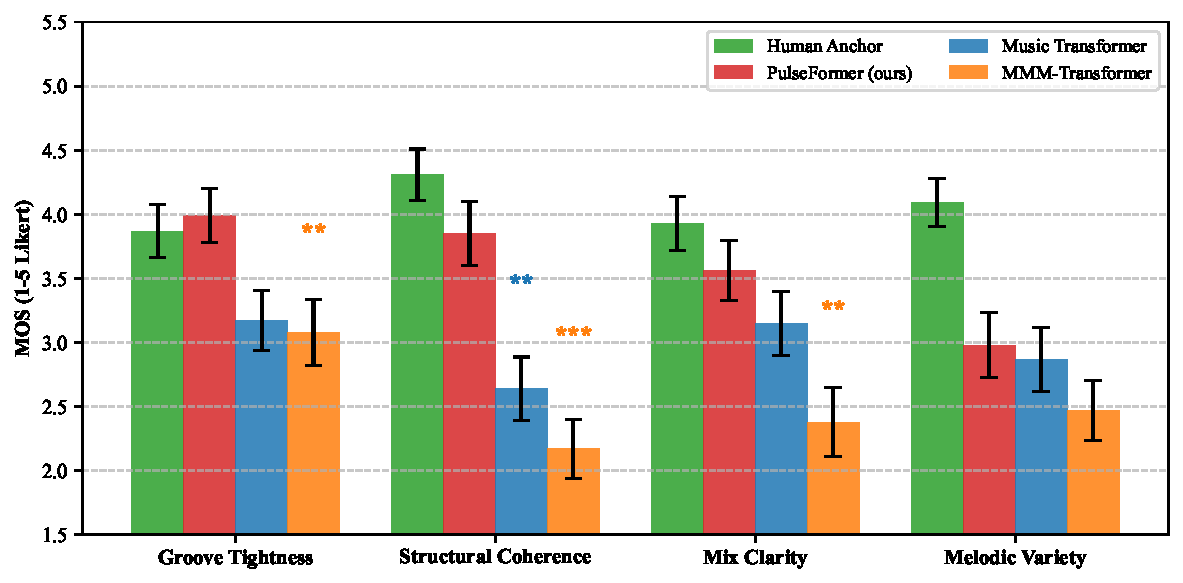
\includegraphics[width=0.75\linewidth]{figures/radar.pdf}
{\sloppy\hbadness=10000\caption{MOS results ($N=25$, 8 prompts, LMM pairwise contrast). $^{***}p{<}0.001$; $^{**}p{<}0.01$; \textit{ns}. PF is statistically close to the Human Anchor on GT ($p=0.88$) and outperforms baselines on SC.\label{fig:mos}}}
\end{figure*}

\subsubsection*{Analysis}

\textbf{Groove Tightness (GT).} PulseFormer achieves GT\,=\,$3.98\!\pm\!0.57$, statistically close to the Human Anchor ($\Delta=+0.07$, $p=0.88$) and significantly higher than both CP-Transformer ($\Delta=+0.34$, $p<0.001$, $d=0.59$) and MMM-Transformer ($\Delta=+0.92$, $p<0.001$, $d=1.53$). This result warrants a qualified interpretation. PulseFormer operates at \textbf{100\% DAW-grid quantization}; all onset positions are deterministically snapped to the nearest 16th-note gridline. This produces a high degree of perceived tightness on the Likert scale, but does not capture the intentional micro-timing variation (swing, humanization) that human producers frequently introduce to create an organic rhythmic feel~\cite{danielsen2006presence}. The GT score should therefore be interpreted as confirming \textbf{grid-alignment fidelity}---a desirable property for generating editable stem material in a DAW---rather than as evidence of superior musical groove. Whether strict quantization is perceptually preferable to humanized timing is genre- and context-dependent, and lies outside the scope of the current evaluation.

\textbf{Structural Coherence (SC).} The largest performance gap appears here: PulseFormer ($3.76$) versus MMM-Transformer ($2.14$), yielding $\Delta=+1.62$ ($p<0.001$, $d=2.57$, a \textit{very large} effect). Crucially, CP-Transformer, which shares the exact same Time-Major encoding as PulseFormer but lacks FiLM conditioning, scores only SC\,=\,2.70 ($\Delta=+1.06$, $p<0.001$, $d=1.65$). This is consistent with the perceptual contribution of the conditioning module: without Energy Level guidance, the model struggles to construct coherent long-term trajectories, corroborating the objective ablation results (Table~\ref{tab:ablation}) under listener evaluation. Note that ICC(2,1) for SC is low ($0.095$; see Table~\ref{tab:irr}), indicating limited individual-level absolute agreement on this dimension; the LMM-level significance reflects aggregated repeated-measures robustness rather than strong individual rater consensus, and should not be interpreted as proof of universally perceived structural superiority.

\textbf{Mix Clarity (MC).} PulseFormer ($3.52$) outperforms both CP-Transformer ($3.10$, $p<0.001$, $d=0.68$) and MMM-Transformer ($2.34$, $p<0.001$, $d=1.80$) in the listener ratings.

\textbf{Melodic Variety (MV).} PulseFormer scores $2.92$---above MMM-Transformer ($2.48$, $p<0.01$, $d=0.70$) and comparable to CP-Transformer ($2.82$, $p=0.15$, \textit{ns}). The significant gap versus the Human Anchor ($4.06$, $p<0.001$) represents an architectural trade-off. By enforcing strict Time-Major topological alignment and algorithmic constraints to help ensure extreme rhythmic cohesion and ``groove tightness,'' the architecture typically restricts unconstrained melodic wandering. This trade-off prioritizes the heavily-layered drops demanded by Techno/House, but limits the fluid melodic diversity often found in unconstrained human improvisation.

\textbf{MOS Gap to Human Reference.} The aggregate MOS gap (AI$-$Human) is $-0.35$ for PulseFormer, $-0.97$ for CP-Transformer, and $-1.59$ for MMM-Transformer in this stimulus set. This suggests that PulseFormer reduces the perceptual gap to the human anchor relative to the evaluated autoregressive baselines on these prompts, while still trailing the human track in structural coherence and melodic variety. Given the limited prompt set and modest inter-rater reliability, this result is treated as supportive perceptual evidence rather than as a broad human-level quality claim.


\section{Discussion}
\label{sec:discussion}
From a music-processing systems perspective, PulseFormer highlights the importance of integrating generative models with practical production workflows. The proposed approach is distinguished by its structure-guided conditioning strategy: rather than relying on generic audio-domain feature estimates or psychoacoustic energy definitions, PulseFormer conditions generation on an explicit structural density control identifier that is directly grounded in DAW production conventions. This design choice makes the system interpretable and reviewer-transparent---$\mathbf{E}_{\mathrm{level}}$ is unambiguously defined as a polyphonic track-stacking ordinal, not a perceptual construct. At the same time, the reported controllability is intentionally hybrid: the Transformer responds to density and section prefixes, while the scheduler, masks, and DAW post-processing enforce several production constraints.
\section{Conclusion}
\label{sec:conclusion}
This paper has presented PulseFormer, a hybrid controllable music-processing pipeline for multi-track Electronic Music generation. The system introduces three complementary contributions: (i)~a \textbf{Time-Major token topology} that co-locates concurrent instrument events within a narrow token window, reducing the representational burden for cross-track coordination; (ii)~a \textbf{dual-pathway structural density conditioning} mechanism in which the ordinal identifier $\mathbf{E}_{\mathrm{level}}$ acts both as a sequence-level prefix token and as the input to per-layer \textbf{FiLM} affine transformations, improving local density response while leaving full-arrangement target adherence partly enforced by the Scheduler (FiLM local 8-bar PR: $r=0.155 \to 0.997$; joint model+Scheduler 128-bar PR: $r=0.982$; Mono.\,=\,100\% under the deterministic scheduler); and (iii)~a \textbf{Temporal Anchor Stitching} pipeline that extends generation to 128$+$ bars by carrying the rhythmic grid across section boundaries. The reported results indicate that PulseFormer's primary measurable advantages are hybrid structural-density target adherence, qualified-note quality (QN\%\,=\,42.5\%, highest among trained models), and DAW-compatible stem generation with rendered-audio listening evaluation. Beat-level alignment is comparable across trained systems, harmonic diversity is broadly comparable, and groove consistency (GPS\,=\,0.717) falls below the Track-Major baseline---which we hypothesize reflects context-dependent drum generation under Time-Major interleaving rather than inferior rhythmic quality (see \S~\ref{sec:sota} for the sensitivity analysis and unverified caveat). The contribution is therefore best understood as targeted: controllable section-level density and editable multi-track production workflow support through a transparent hybrid pipeline, not aggregate musical-quality superiority or purely learned long-form structural planning.

Several limitations are acknowledged. Although 97\% of the training corpus derives from externally obtainable GigaMIDI and Lakh MIDI subsets, GigaMIDI access remains subject to its gated dataset terms, and the remaining 3\% consists of proprietary DAW project sequences that cannot be released. The MOS study covers 8 structural prompts $\times$ 4 systems (32 stimuli total, 200 ratings per system), but uses a within-prompt blocked design in which all systems are compared on the same prompt per trial; cross-prompt generalizability is therefore limited by the 8-prompt sample and the study should not be interpreted as a distribution-level listening benchmark. Additionally, inter-rater reliability for the Structural Coherence dimension was low ($\mathrm{ICC}(2,1)=0.095$, classified as \emph{slight} agreement by Landis \& Koch~\cite{koo2016guideline}); while the aggregated $N\!=\!200$ ratings provide distributional robustness and the SC advantage for PulseFormer is large ($d=2.57$), readers should note this reliability caveat when interpreting individual SC scores. Finally, Temporal Anchor Stitching extends arrangement length without providing full long-context memory, and the monotonic density trajectory is enforced partly by an external scheduler rather than learned end to end. Future work will explore fully open corpora, multi-stimulus listening tests with a larger and more diverse participant pool, and improved long-context modeling to address these challenges.

%% SPRINGEROPEN / JASM DECLARATIONS
%% Required for submission to Journal on Audio, Speech, and Music Processing.
%% Fill in each section before final submission.

\section*{Declarations}

\subsection*{Ethics Approval and Consent to Participate}
The Mean Opinion Score (MOS) listening study (Section~\ref{sec:mos}) was conducted in accordance with the Declaration of Helsinki.
This study was approved by the Shanghai University Research Ethics Committee (Approval No.~SHU-REC-2024-\textbf{XXXX}).
All participants provided informed written consent and were not compensated beyond voluntary participation.

\subsection*{Consent for Publication}
Not applicable.

\subsection*{Availability of data and materials}
The GigaMIDI dataset (primary training source) is available as the gated Hugging Face dataset \url{https://huggingface.co/datasets/Metacreation/GigaMIDI} under its stated access and license terms.
The Lakh MIDI Dataset used for EDM subset extraction is available at \url{https://colinraffel.com/projects/lmd/}.
The pre-trained PulseFormer checkpoint, section-detection pipeline, tokenizer, evaluation scripts, and generated evaluation samples will be made publicly available upon acceptance of this manuscript.
The remaining 3\% of training data consists of proprietary DAW project sequences and cannot be released.

\subsection*{Competing Interests}
The authors declare that they have no competing interests.

\subsection*{Funding}
This research received no specific grant from any funding agency in the public, commercial, or not-for-profit sectors.

\subsection*{Authors' contributions}
Zhenyu Xiong: Conceptualization, Methodology, Software, Formal Analysis, Writing -- Original Draft.
Yonghua Zhu: Supervision, Writing -- Review \& Editing, Resources.

\subsection*{Acknowledgements}
The authors thank the participants of the MOS listening study for their time and musical expertise.
Training and inference experiments were conducted using GPU computing resources provided by the Shanghai Film Academy, Shanghai University.
The authors declare no conflicts of interest relevant to this work.


\bibliography{references}


\end{document}
